\chapter{Tools and Methodologies}
This chapter describes tools that can be handled to validate Java applications and methodologies that can be applied depending on different validation purposes.

The first section is a presentation of the JACK tool,
\marginpar{TODO}
\section{JACK}
This section presents the Java Applet Correctness Kit (or \JACK).
This tool, already briefly described in \cite{BRL-JACK}, is
a formal tool that allows one to prove properties on Java programs
using the Java Modeling Language \cite{Leavens-Baker-Ruby03} (JML).
It has been developed initially by Gemplus, and since 2003 by INRIA
in the context of a bilateral collaboration with Gemplus, and then
in the context of the INSPIRED project.


It generates proof obligations allowing to prove that the Java code
conforms to its JML specification.  The lemmas are translated into an
internal formula language called JPOL (Java/Jack Proof Obligation
Language). Then JPOL verification conditions are translated into
different prover language, namely Coq, PVS, Simplify and the B
language \cite{bbook}, allowing to use the automatic provers Simplify
and the provers developed within the B method and interactive provers
like the Coq proof assistant, PVS or Click'n'Prove.

 But the tool is not yet another lemma generator for Java, since it
 also provides a lemma viewer integrated in the eclipse
 IDE\footnote{\texttt{http://www.eclipse.org}}, which is one of the
 most commonly used IDE for Java developers.  This allows to hide the
 formalisms used behind a graphical interface.  Lemmas are presented
 to users in a way they can understand them easier, by using the Java
 syntax and highlighting code portions to help the
 understanding. Using \JACK, one does not have to learn a formal
 language to be confident on code correctness.

 The remainder of the section is organized as follows.  Subsection
 \ref{JavaAppletCorrectnessKit} presents the architecture and the main
 principles of the tool we have developed.  Subsection~\ref{JPOL}
 presents the Java/Jack Proof Obligation Language (JPOL).
 Subsection~\ref{Industrialisation} describes more precisely the
 innovative parts of the tool and explains why we consider it as
 accessible to any developers.

\subsection{Foundations}
\label{JavaAppletCorrectnessKit}
 The main design goals were the following:
 \begin{itemize}
 \item it should provide an easy accessible user interface, that enables average Java programmers to use the tool
 without too much difficulties (in contrast to for example \LOOP). This interface is
described section \ref{Industrialisation};
 \item it should provide a high degree of automation, so that most proof obligations can be discharged without user
 interaction. Only in this way, the tool can be effectively used by non-expert users, which is necessary if we want that
 formal methods will ever be used in industry. 
 \item it should provide high correctness assurance: at the moment the prover says that a certain proof obligation
is satisfied, it should be possible to trust this without any reservation. Nevertheless
the tool is not formally developed, as \LOOP\ is. It implements, in Java, a weakest precondition calculus that
generates lemmas without user interaction. We cannot prove that those lemmas are necessary and sufficient to
ensure the correctness of the applet but the tool is designed in this way;
 \item it should be relatively independent of any particular prover, so that if the use of another prover is
 required (for example by a certification institute) it is relatively easy to adapt the tool accordingly.
\end{itemize}

 This section presents the tool architecture and its principles.
\subsubsection{Architecture}
\begin{figure}[tp]
 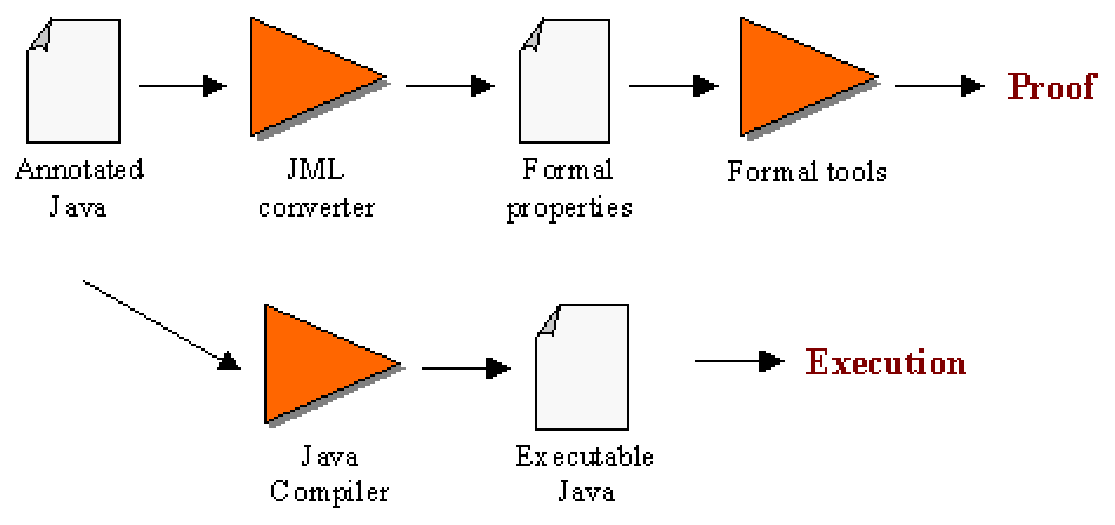
\psfig{file=fm03/image002.eps,width=14cm}
 \caption{\JACK\ architecture}
 \label{JACKarchitecture}
\end{figure}
 Figure \ref{JACKarchitecture} presents an overview of the \JACK\
 architecture.  \JACK\ consists of two parts: a converter (a lemma generator) from
 Java source annotated with JML into JPOL lemmas, and a viewer that
 allows developers to understand the generated
 lemmas.  The viewer is integrated in an IDE and is described more precisely in section
 \ref{Viewer}.  This part focuses on the converter.

 The \JACK\ converter converts a Java class into a JPOL model and allows to
 prove properties. 
 Our goal is to prove properties on source files written with the Java
 language.  To reach this goal, one has to know how to ``translate'' a
 Java source file in formal lemmas.  

\begin{figure}[p]
 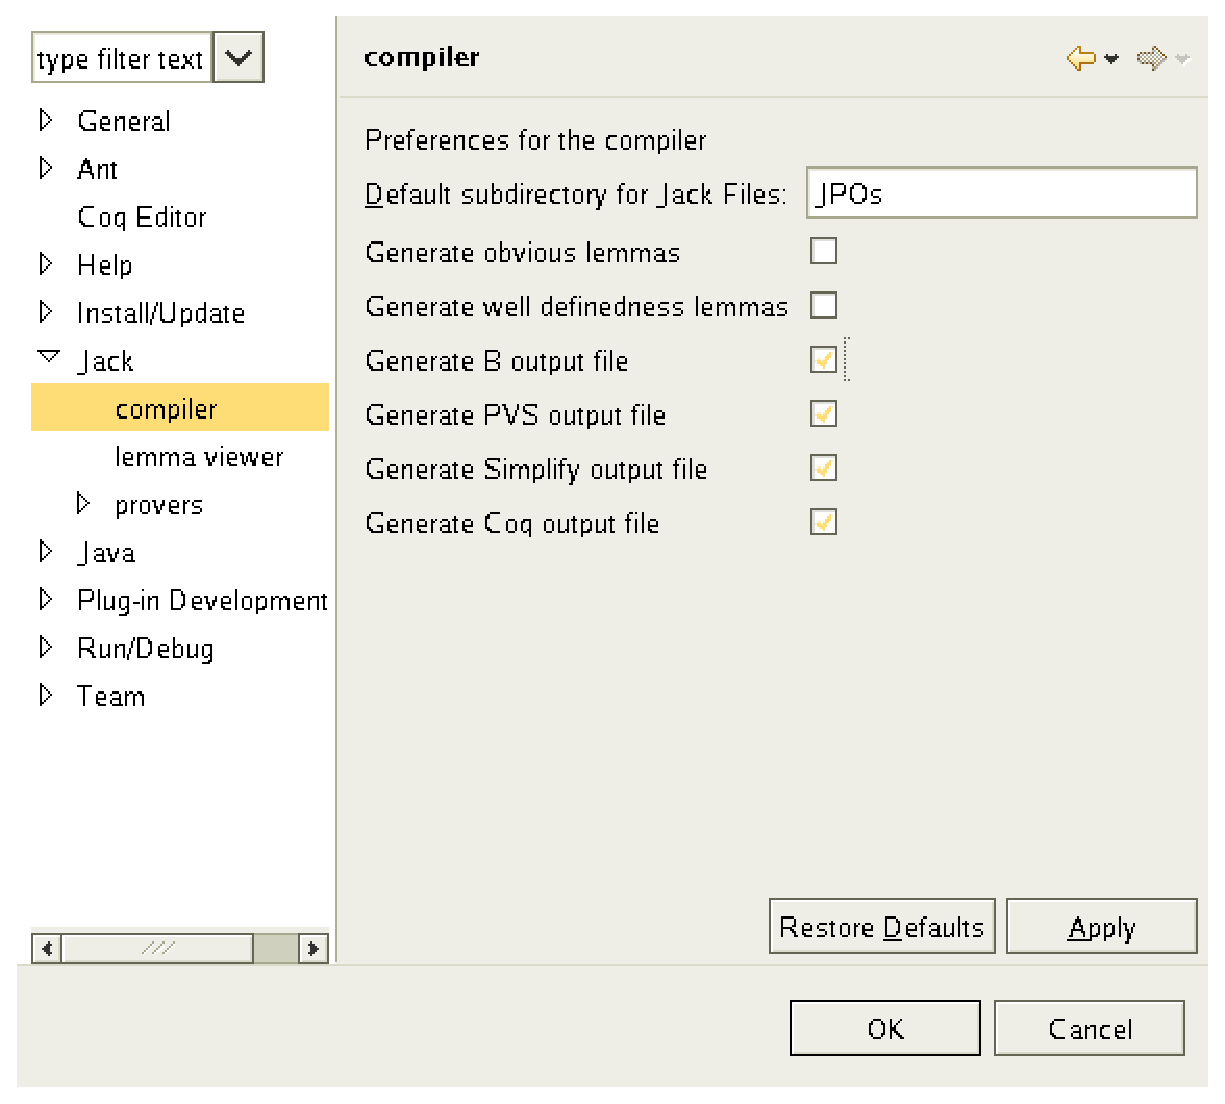
\psfig{file=fm03/preferences-compiler.eps,width=14cm}
 \caption{\JACK\ compiler preferences page}
 \label{JACKcompprefpage}
\end{figure}
 The JML annotations are Java boolean expressions without side
 effects.  Thus, they are easily translated in logical formulas: Java operators are
 translated into functions. For example, shift left (\texttt{<<}) is
 translated into a function associating an integer to a pair of
 integer.  From those translated annotations and the methods code,
 lemmas can be generated automatically.

 From the start, taking into account
 experiences in lemma generation for B machines, we have tried to
 implement a Weakest Precondition (WP) calculus to automate lemma
 generation.  Huisman, in \cite{Huisman:PhD}, presents how the
 classical Hoare logic can be completed to allow the generation of
 lemmas in the context of Java.  The Java statements contain different
 features like control-flow breaks.  So, the classical WP calculus
 should be completed to deal with them.

 Moreover, JML should be lightly upgraded to allow fully automated proof obligation generation.
 Notably, to
 automate lemma generation for the loops, we have had to extend
 the JML language with new keywords: \texttt{loop\_modifies} and \texttt{loop\_exsures}.
 The \texttt{loop\_modifies} keyword allows us to declare the variables modified in
the body of the loop, as it is done for the methods. During the WP calculus, it is necessary to universally
quantify the loop invariant with those variables, and since they cannot be automatically calculated, one has to
specify them.
 The \texttt{loop\_exsures} allows us to specify the exceptional behavior of a loop. It is not necessary to apply
the WP calculus but it can improve the understandability of the specification.

 The two main drawbacks of the WP calculus are the loss of information and
 potential exponentional explosion.  After lemmas have been generated,
 it is often difficult to understand from which part of the code they
 are derived.  To bypass this issue, program flow information is
 associated to each lemma.  This information is used in the viewer
 to associate an execution path to each lemma. This feature is described in the next section.

 Exponentional explosion remains a problem.  Different solutions exist
 to avoid it.  As the WP calculus can be considered as a brute
 force concept, trying to expand all the path of the methods,
 solutions are always based on interaction to reduce this brute force
 by introducing intelligence in the process.

 A simple solution is to require users interaction during lemma
 generation in order to cut unsatisfiable branches.  Rather than introducing
 interaction during generation, another solution is to allow to add
 special annotations in the source code to introduce formulas that are
 taken into account at generation to simplify the lemmas.
 The solution adopted in \JACK\ is to allow to specify blocks. An exponentional explosion usually occurs
in a method with many sequenced branched statement ({\tt if, switch}, etc.) Such methods usually perform
different distinct sequenced treatments.
 Figure \ref{Specified_block} presents the skeleton of such a method. Specifying a block (here the second part
of the method) allows to cut proof obligation generation. This corresponds, in fact, to the simulation of a
method call.
\begin{figure}[htp]
{\tt
\begin{tabbing}
 \hspace{3 cm} \=m()\= \ \{ \\
 \> \> \vdots \\
 \> \> if () \{ $\hdots$ \} \\
 \> \> else \{ $\hdots$ \}   \\
 \> \> \vdots                   \\
 \> \> /*\=@ modifies {\it variables}  \\
 \> \> \> @ ensures {\it property} \\
 \> \> \> @\=*/ \{ \\
 \> \> \> \> \vdots \\
 \> \> \> \> if () \{ $\hdots$ \} \\
 \> \> \> \> else \{ $\hdots$ \}   \\
 \> \> \> \> \vdots                   \\
 \> \> \ \} \\
 \> \> \}
\end{tabbing}
}
 \caption{Specified block}
 \label{Specified_block}
\end{figure}

 With those extensions to the JML language, we are able to obtain a fully automated proof obligation generation.
That is the first step to reach user approval. The second one is to propose an access to those lemmas in a
``Java style'', this is described in the next section.

\subsection{User Interface}
\label{Industrialisation}
JML has the advantage of being a language that can be rapidly and
easily learned and used by developers. One can consider that using a
prover is not so easy. Nevertheless formal activities like modeling
and proving should not be reserved to experts. To demonstrate this
concept, we provide a prover interface understandable to non-experts
in formal methods.

In order to simplify the modeling activity with the JML language, our
interface requirements are:
\begin{itemize}
 \item to be integrated with other tools used by developers, and
 \item not to require the developer to use a mathematical formalism,
    but hide the mathematical formalism under a ``Java'' view.
\end{itemize}
Compared to other formal tools using the JML language, the efforts on
the user interface and integration within the development
environment is probably the main strength of \JACK, as is the fact
that the underlying mathematical formalism is not exposed to the
user.
\paragraph{Integration in developers environment}
 Java developers are used to develop using integrated development
 environments (IDE).  Those IDEs provide many features useful during
 the development process.  Integrating the tool in such IDEs allows
 the user to work in a familiar environment.  This leads both to
 better acceptance of the tool, and to a reduced learning curve.
 Currently, \JACK\ is integrated within the eclipse IDE.  It could
 however be ported to other IDEs, and a standalone version that does
 not require an IDE also exists.

 Another constraint has to be taken into account to obtain developer
 agreement: it is the tool's responsiveness.  The tool has to be used
 interactively, with a debugger spirit: it should not require the
 developer to wait for a long time.  Lemma generation takes, in
 realistic examples, less
 than one minute. %(see Section \ref{Case Study} for metrics).
 Nevertheless, the automatic proof of lemmas is not such a reactive
 activity. Thus, the tool provides a feature that allows to schedule
 proof tasks in order to optimize proof time (see paragraph
 \ref{Support for automatic proof}).


%Several other minor features are available to integrate within the
%development cycle, for example, reports on the status of the project
%can be generated as Microsoft Excel files.
\paragraph{Lemma Viewer}
\begin{figure}[p]
 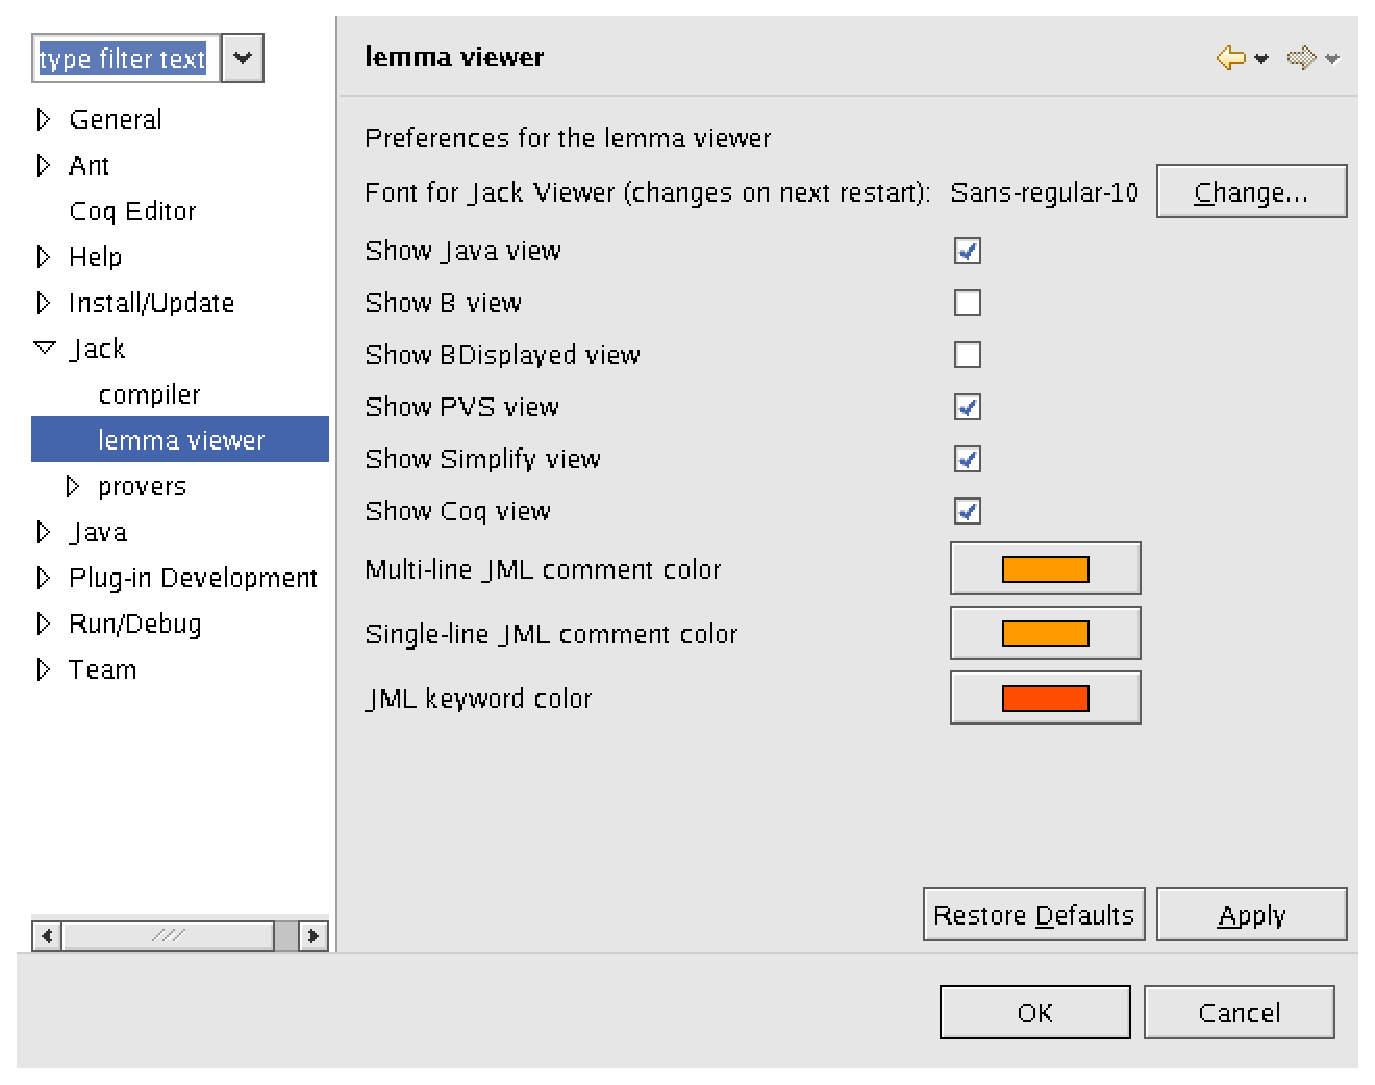
\psfig{file=fm03/preferences-editor.eps,width=14cm}
 \caption{\sc \JACK\ lemma viewer preferences page}
 \label{JACKlemviewprefpage}
\end{figure}
\label{Viewer}
One of the most important points of \JACK\ is that it does not require
developers to learn a mathematical language.  Although lemmas are
generated, those lemmas are not directly displayed to the user.

Instead, we provide the user with a graphical view (Figure \ref{Viewer image}) of the lemma.
 The viewer displays
 \begin{itemize}
  \item information concerning the current proof status;
  \item the class methods with their lemmas;
  \item the source code;
  \item and the currently selected lemma (goals and hypotheses with JPOL and prover language translations).
\end{itemize}
 Within a method, each execution path corresponds to a case.
 Possibly, several lemmas are associated to each case.
 When a case is selected, the corresponding execution path is highlighted.
 When a lemma is selected, its views are displayed.
\subparagraph{Path highlighting}
The source code of the program considered is displayed, and the
path within the program that leads to the generated proof obligation
is highlighted.

\begin{figure}[p]
 \epsfig{file=fm03/jack01.eps,width=15cm}
 \caption{\sc Viewer integrated in eclipse}
 \label{Viewer image}
\end{figure}

Different highlighting colors are used to represent this path:
\begin{itemize}
\item green indicates that the corresponding instruction has been
   executed normally;
\item blue indicates that the corresponding instruction has been
   executed normally, and that additional information is
   available. For instance, the condition of an \texttt{if} construct will
   usually be displayed in blue with additional information indicating
   if the condition has been considered as true or false;
\item red indicates that the corresponding instruction was supposed to
   raise an exception when it has been executed in the case
   considered.  Additional information are also provided indicating
   the exception that has been raised.
\end{itemize}
The part of the specification (invariant or post-condition) that is
involved in the current lemma is also highlighted.  Highlighting the
part of the source code involved in the proof obligation allows to
quickly understand the proof obligation, and allows the user to treat
the proof obligations as execution scenarios of the program.
\subparagraph{Java presentation of lemmas}
The hypothesis and goals of the current lemma are also displayed. As
the conversion mechanism into provers language may be hard to follow, especially by
non-experts, the internal representation used by the tool is used to
present the hypothesis and goals in a Java representation. That is,
all the variables are displayed using the Java dotted notation, and
the Java operators are used instead of their corresponding function.

However, such a translation may be more complicated when operators that
have no Java or JML equivalent constructs are used.  


 However, although the Java view is able to handle some internal
 representation constructs that do not have direct Java or JML
 equivalent constructs, there are still constructs that cannot be
 translated, and for which a Java notation is hard to define. For
 instance some set operators cannot be translated in a generic way.

\subsubsection{Support for verification}
Apart from displaying the generated proof obligations, \JACK\ also
provides support for validating those proofs, as detailed hereafter.
\subparagraph{Support for automatic proof}
\label{Support for automatic proof}
 A point that should not be taken lightly is the time taken by
automatic proof: generating proof obligations for industrial size
applications will generate thousands of proof obligations.

Typically, those proofs can be quite lengthy, and it is necessary that
the user is not obliged to wait for proofs to finish.

To achieve this, \JACK\ provides an independent proof view, where
files can be queued in order to be submitted to the prover. Thus, the
proofs are performed as soon as possible, possibly during the night,
allowing the user to focus on cases inspection.

\subparagraph{Support for interactive proof}
Although the automatic prover allows discharging many proof
obligations, it cannot discharge all the proof obligations. Thus, the
remaining proof obligations have to be verified manually.

Currently, developers are not supposed to handle this task, but to
delegate it to a team of experts that would perform the proofs using
the interactive prover of the \texttt{Atelier B} tool, emacs with PVS
or the Coq editor.


\subparagraph{Checking proof obligations}
Additionally to the ``\textit{proved}'' and ``\textit{unproved}''
states, \JACK\ can also differentiate ``\textit{checked}'' proof
obligations. Checked proof obligations correspond to proof obligations
that are not formally proved, but have been manually verified.

Checking proof obligations is performed by the user to indicate that
he has read and understood the proof obligation and has confidence
that it is correct. Although the checked state provides no formal
guarantee on the correctness of the proof obligations, it still
provides valuable information on the state of a project.

The checked state of the proof obligations can be used in different
ways:
\begin{itemize}
\item To flag cases as already seen in order to start an interactive
   proof only if we are pretty sure that the cases are correct, and
\item In some cases, when a full correctness assurance of the program is not
   required, we may accept that not all the proof obligations are
   formally proved. In that case, it may however, be required that all
   the proof obligations have been checked.
\end{itemize}
In order to minimize verification time, one can assure that checked
proof obligations remain unchanged through subsequents runs of the
proof obligation generator---otherwise the time spent to inspect the
proof obligation and to ensure manually that it is correct would be
lost. 


\subsection{Case study}
\label{Case Study}
% Tableau avec chiffres, etc...
To test \JACK, we have developed a little banking application.  This section presents different metrics
concerning the evaluation of the tool on this package.
\begin{table}
 \begin{tabular}{|l|c|c|c|c|c|c|c|} \hline
 Classes & Java & JavaDoc & JML & Proof & Automatic & Time to PO & Time to \\
  & lines & lines & lines & obligations & proof & generate (s) & prove (s)\\  \hline
 Transfert\_src  & 116 & 34 & 150 & 359 & 91\% & 22,5 & 238 \\
 AccountMan\_src & 105 & 51 & 236 & 269 & 82\% & 12,7 & 195 \\
 Currency\_src   &  93 & 20 &  28 &  50 & 96\% &  7,6 &  17 \\
 Balance\_src    &  64 & 38 &  58 & 335 & 95\% & 16,5 & 191 \\
 Spending\_rule  &  40 & 33 &  62 &  42 & 67\% & 13,6 & 217 \\ \hline
 \end{tabular}
\caption{banking applet metrics}
\label{MetricsTable}
\end{table}
Different remarks can be made from Table \ref{MetricsTable}, concerning the cost of adding JML annotations, the
performance of the tool, as well as the cost associated to the proof.
\paragraph{Cost of the annotations}
A first remark concerns the cost of the annotations.  The metrics given here only concern the number of lines
but one can see that the documentation size (JavaDoc and JML) is one and half greater than the code size.  So,
writing  the JML specification seems to be a costly activity.  This remark can be moderated by two points: this
development was the first that we made, and annotations were added to already existing code. So it suffers from
its lack of abstraction, and the annotations are really verbose. Moreover the time to specify is to be compared
to the time to develop test data.
\paragraph{Responsiveness}
The automatic phases are quite responsive with some seconds to generate proof obligations.  The automatic proof
is not as cheap as the proof obligation generation and takes a few minutes. However, this still remains
acceptable, since it is a non-blocking task that does not require users to wait for its completion.

For larger applets, it is however expected that the time required for the automatic proof will significantly
increase.
\paragraph{Proof}
The automatic proof rating is much good.  It is quite greater than the usual value for a B development (around
80\%).  This is mainly due to the fact that we used this applet as a test applet for extending the prover. So,
as a side effect, the automatic prover is customized for this special applet.

Nevertheless, after automatic proof step, there remain 111 lemmas to prove using the Atelier B interface.  An
expert needs between 4 and 5 days to prove them.

\subsection{Perspectives}
\label{Perspectives}
 At the moment, we have developed a prototype that is becoming a
 usable tool.  We are beginning experimentation outside the lab.  But
 we are considering that there are still many points where the
 approach can be improved.
%\subsection{JML Subset considered}
% JACK currently handles a subset of JML corresponding to lightweight
% specifications.  Future work should improve that subset by allowing
% to use a larger subset of JML including full fledged behavior
% specifications and pure method calls.

\subsubsection{Interactive proof cost}
 Currently, the interactive proof support is rather limited.  Thus,
 proving the remaining proof obligations requires users to directly
 use the \texttt{Atelier B} tool interactive prover.  Such a task can
 be tedious, since the B representation of the generated proof
 obligations can be hard to follow.  Different perspectives exist to
 reduce the interactive proof cost.

% AR: remplac� non-expert par Java: en effet je trouve que �a serais
% plus pratique m�me pour un expert.
\paragraph{Java interface}
 Although full interactive proof will still be reserved to experts,
 providing an interface to the \texttt{Atelier B} interactive prover
 allowing to perform proofs by directly using the Java syntax would
 greatly improve the productivity of those experts.  A first step
 would be to extend the Java view used to display the lemmas.

\paragraph{Test Activity}
 Another way to reduce interactive proof activity is to balance it
 with testing activity.  Methods where lemmas are not automatically
 proved could be tested.  Using \texttt{JmlJunit} can be a good way to
 generate test skeleton on certain cases.  A perspective is to
 integrate \texttt{JmlJunit} in our environment in manner to propose
 different validation level (full proof, proof mixed with test, etc).

\paragraph{Counter-example}
 Another idea to reduce the cost of false lemma detection is to
 provide counter-example when it is possible.  \ESC\ already tempts to
 give such counter-examples.  Studies on that subject could give
 results helpful for developers to understand errors on the code or on
 the specifications.

\subsubsection{Allowing expressions in the target formal language}
Currently, \JACK\ can be seen as a proof-obligations generator from
JML annotated Java programs to B lemmas.  A possible extension would
be to add different target languages for lemma generation, for
instance Coq or PVS. Such extension would allow using different
provers for different lemmas.  On the other side, it is also possible
to enrich the JML specification by adding inline expressions or
variables in a target language of the lemma generator. 
Such an extension would have a role similar to Java ``native methods''
at a specification level. That is, allowing to describe in a
lower-level language things that cannot be described in JML (or that
cannot be described efficiently from a proof point of view).

We are currently investigating such extension mechanisms, that would
allow adding different languages for such use without having to modify
the weakest-precondition calculus core.

\subsection{Conclusion}
\label{Conclusion}
 The presented work allows formal methods experts to prove Java applet correctness.
 Moreover, it allow Java programmers to obtain an high assurance on their code correctness.
 This leads to the most important point:
it allows non-experts to venture into the formal world.  This is a necessary starting point for such validation
techniques to be widely used.

  The tool has been developed following a main
 objective: let Java developers validate their own code.  We claim
 that JML is well suited to express low level design and conception
 choices and that usage of \JACK\ can replace effectively unitary tests,
 giving developers the means to furnish code with good quality
 and non ambiguous documentation.

 Taking benefits from recent research on Java program validation, we have
 developed an automated tool that generates lemmas from Java classes
 annotated with JML.
 The \JACK\ principles are not really different from the \LOOP\
 team choices.  Nevertheless, one can highlight some important
 differences.
 The \LOOP\ tool describes formally Java semantics and the WP-calculus rules are applied by the prover.
 The main advantage is that the rules have been proved sound with regards to the semantics in the theorem prover.
 Our point of view, is more pragmatic: lemma are generated automatically, using
 Java developed rules that can only be checked by usual validation: test, code-inspection.
 The soundness of the tool cannot be formally proved but on the other hand a big effort is done to present
 lemmas to users in a way that he can understand them and verify
 that they are valid.

 The tool is fully integrated in the eclipse IDE
 and presents lemmas in a visual way that allows developers to form their
 opinion on the lemma validity.  An automatic prover discharges an
 important part of the lemmas.  The remaining lemmas have to be proved
 using the prover interface.  Often, this task cannot be done by developers.
 Different ways are studied to bypass it: expert support, test case
 generation, counter-example detection, etc.

 We are now experimenting on real industrial products.  We are
 trying to collect metrics in order to prove that this kind of
 validation is cost-saving, especially when the cost of testing is
 taken into account.


\section{Security property propagation}

%\input BML/cmdBML.tex

\newcommand{\code}{\textit{code}}
\newcommand{\indexComp}{\textit{index}}





%\section{Introduction} \label{bcsl}
This chapter presents the bytecode level specification language, called for short BML and a compiler from a
 subset of the high level Java specification language JML to BML which from now we shall call \JMLtoBML. 
The chapter is organized as follows.
 In section \ref{BCSLprelim}, we give an overview of the main features of JML. A detailed overview of BML is given in section \ref{BCSLgrammar}.  
  As we stated before, we support also a compiler from the high level specification language JML into BML. The 
 compilation process from JML to BML is discussed in section  \ref{BCSLcompile}.
 The full specification of the new user defined Java attributes in which the JML specification is compiled is given in the appendix.





\subsection{High-level Security Properties for Applets}  \label{SecHighLevelSecProp}

% However, as these applications should be
%able to share information, this raises big challenges for the security
%of smart cards. Moreover, one would like that a smart card holder
%dynamically can download new applications, while the card is already
%out in the field, which of course raises even more security
%issues. 

Over the last years, smart cards have evolved from proprietary into
open systems, making it possible to have applications from different
providers on a single card. To ensure that these applications cannot
damage the other applications or the card itself, strict security
policies---expressed as high-level security properties---must be
obeyed.  Such properties are high-level in the sense that they have
impact on the whole application and are not restricted to single
classes. Below we will present several examples. It is important to
notice that we restrict our attention to source code-level security of
applications.

The properties that we consider can be divided in several groups,
related to different aspects of smart cards. First of all there are
properties dealing with the so-called \emph{applet life cycle},
describing the different phases that an applet can be in. Many actions
can only be performed when an applet is in a certain phase. Second,
there are properties dealing with the transaction mechanism, the Java
Card solution for having atomic updates. Further there are properties
restricting the kind of exceptions that can occur, and finally, we
consider properties dealing with access control, limiting the possible
interactions between different applications. For each group we present
some example properties. For all these properties encodings into JML
annotations exist.

We would like to emphasise that there exist many more
relevant security properties for smart cards, for example specifying
memory management, information flow and management of sensitive
data. Identifying all relevant security properties for smart cards,
and expressing them formally, is an important ongoing research issue.
 

\paragraph {Applet life cycle}

A typical applet life cycle defines phases as {\it loading},
{\it installation}, {\it personalisation}, {\it selectable},
{\it blocked} and {\it dead}
(see \emph{e.g.}~\/\cite{MarletL01}).  Each phase corresponds to a
different moment in the applet's life. First an applet is loaded on
the card, then it is properly installed and registered with the Java
Card Runtime Environment. Next the card is personalised,
\emph{i.e.}~all information about the card owner, permissions, keys
\emph{etc.} is stored. After this, the applet is selectable, which means
that it can be repeatedly selected, executed, and deselected. However,
if a serious error occurs, for example there
have been too many attempts to verify a pin code, the card can get
blocked or even become dead. From the latter state, no recovery is
possible.

In many of these phases, restrictions apply on who can perform
actions, or on which actions can be performed. These restrictions give
rise to different security properties, to be obeyed by the applet.

\begin{quote}
\textbf{Authenticated initialisation} Loading, installing and 
personalising the applet can only be done by an authenticated
authority.\smallskip\\
\textbf{Authenticated unblocking} When the card is blocked,
only an authenticated authority can execute commands and possibly
unblock it.\smallskip\\
\textbf{Single personalisation} An applet can be
personalised only once.
\end{quote}


\paragraph {Atomicity}

A smart card does not include a power supply, thus a brutal retrieval
from the terminal could interrupt a computation and bring the system in
an incoherent state. To avoid this, the Java Card
specification prescribes the use of a transaction mechanism to
control synchronised updates of sensitive data. A 
statement block surrounded by the methods \texttt{beginTransaction()} and
\texttt{commitTransaction()} can be considered atomic.
If something happens while executing the transaction (or if
\texttt{abortTransaction()} is executed), the card will
roll back its internal state to the state before the transaction was
begun.

To ensure the proper functioning and prevent abuse of this mechanism,
several security properties can be specified.

\begin{quote}
\textbf{No nested transactions} Only one level of transactions
is allowed.\smallskip\\
\textbf{No exception in transaction} All exceptions that may be thrown
inside a transaction, should also be caught inside the
transaction.\smallskip\\
\textbf{Bounded retries}
No pin verification may happen within a transaction.
\end{quote} 
The second property ensures that the \texttt{commitTransaction} will
always be executed. If the exception is not caught, the
\texttt{commitTransaction} would be ignored and the transaction would
not be finished. The last property excludes pin verification within a
transaction. If this would be allowed, one could abort the transaction
every time a wrong pin code has been entered. As this rolls
back the internal state to the state before the transaction was
started, this would also reset the retry counter, thus allowing an
unbounded number of retries. Even though the specification of the Java
Card API prescribes that the retry counter for pin verification cannot
be rolled back, in general one has to check this kind of properties.

\paragraph{Exceptions}

Raising an exception at the top level can reveal
information about the behaviour of the application and in principle it
should be forbidden. However, sometimes it is necessary to pass on
information about a problem that occurred. Therefore, the Java
Card standard defines so-called ISO exceptions, where a pre-defined
status word explains the problem encountered. These exceptions are the
only exceptions that may be visible at top-level; all other exceptions
should be caught within the application.

\begin{quote}
\textbf{Only ISO exceptions at top-level}
No exception should be visible at top-level, except ISO
exceptions.
\end{quote}

\paragraph {Access control} 

Another feature of Java Card is an isolation mechanism between
applications: the firewall. The firewall ensures that several
applications can securely co-exist on the same card, while managing
limited collaboration between them: classes and interfaces defined in
the same package can freely access each other, while external classes
can only be accessed via explicitly shared
interfaces. Inter-application communication via shareable interfaces
should only take place when the applet is selectable, in all other
phases of the applet life cycle only authenticated authorities are
allowed to access the applet. 
\begin{quote}
\textbf{Only selectable applications shareable} An application is accessible
via a shareable interface only if it is selectable.
\end{quote}


\paragraph*{Architecture}

\begin{figure}[pht]
\begin{center}
\epsfig{file=isaac/architecture.eps, width=9cm}
\end{center}
\caption{\sc Tool set for verifying high-level security properties}\label{FigArch}
\end{figure}



Figure~\ref{FigArch} shows the general architecture of the tool set
for verifying high-level security properties. Our annotation generator
can be used as a front-end for any tool accepting JML-annotated Java
(Card) applications. As input we have a security property and a Java
Card applet. The output is a JML Abstract Syntax Tree (AST), using the
format as defined for the standard JML parser. When pretty-printed,
this AST corresponds to a JML-annotated Java file. From this
annotated file, JACK generates appropriate proof obligations to check
whether the applet respects the security property.

\paragraph*{Automatic Generation of Annotations}
The purpose of this section is to provide a brief description of the
weaving phase, \emph{i.e.}~how the core-annotations are propagated
throughout the applet. We define functions \textsf{mod}, \textsf{pre},
\textsf{post} and \textsf{exc\-post}, propagating assignable clauses,
preconditions, postconditions and exceptional postconditions,
respectively. These functions have been defined and implemented for
the full Java Card language, but to present our ideas, we only give
the definitions for a representative subset of statements: statement
composition, method calls, conditional and \texttt{try}-\texttt{catch}
statements and special set-annotations. We assume the existence of
domains \textsf{MethName} of method names, \textsf{Stmt} of Java Card
statements, \textsf{Expr} of Java Card expressions, and \textsf{Var}
of static ghost variables, and functions \textsf{call} and
\textsf{body}, denoting a method call and body, respectively.

All functions are defined as mutual recursive functions on method
names, statements and expressions. When a method call is encountered,
the implementation will check whether annotations already have been
generated for this method (either by synthesizing or weaving). If not
it will recursively generate appropriate annotations. Java Card
applets typically do not contain (mutually) recursive method calls,
therefore this does not cause any problems. Generating appropriate
annotations for recursive methods would require more care (and in
general it might not be possible to do without any user interaction).


\paragraph{Propagation of assignable clauses}
First we define a function \textsf{mod} that propagates
assignable clauses for static ghost variables.

%Different from the standard JML set of modified variables in a method, that takes into account  both JML and 
%Java variables, we keep track only of JML ghost static variables. For our purposes this is sufficient because the generated pre- and postconditions involve only ghost variables.
\begin{definition}[\textsf{mod}]We define functions
%\[
%\begin{array}{rcl}
\(\mathsf{mod} \colon \mathsf{MethName} \rightarrow
\mathcal{P}(\mathsf{Var})\), 
\(
\mathsf{mod}  \colon  \mathsf{Stmt}   \rightarrow
\mathcal{P}(\mathsf{Var}) \), and 
\(\mathsf{mod}  \colon  \mathsf{Expr}   \rightarrow  \mathcal{P}(\mathsf{Var})\)
%\end{array}
%\]
by rules like (where \(m,n\,\colon\mathsf{MethName}\),
\(s_1,s_2\,\colon\mathsf{Stmt}\), \(c\,\colon\mathsf{Expr}\) and \(x\colon\mathsf{Var}\)):
\[
\begin{array}{rcl}
\mathsf{mod}(m) & = & \mathsf{mod}(\mathsf{body}(m)) \smallskip \\
\mathsf{mod}(s_1 \mathtt{;} s_2) & = & \mathsf{mod}(s_1) \cup \mathsf{mod}(s_2)\\
\mathsf{mod}(\mathsf{call}(n)) & = &  \mathsf{mod}(n) \\
\mathsf{mod}(\mathtt{if\:(} c \mathtt{)\:} s_1 \mathtt{\:else\:} s_2)
&=& \mathsf{mod}(c) \cup \mathsf{mod}(s_1) \cup \mathsf{mod}(s_2)\\
\mathsf{mod}(\mathtt{try\:} s_1 \mathtt{\:catch\:(} E \mathtt{)\:}
s_2) & = & \mathsf{mod}(s_1) \cup \mathsf{mod}(s_2)\\
\mathsf{mod}(\mathtt{set\:}x \mathtt{\:=\:} c) & = &  \{ x \} 
\end{array}
\]
\end{definition}


\paragraph{Propagation of preconditions}
Next, we define a function \textsf{pre} for
propagating preconditions. This function analyses a
method body in a sequential way---from beginning to end---computing
which preconditions of the methods called within the body have to be
propagated. To understand the reasoning behind the definition, we will
first look at an example. Suppose we are checking the \textbf{No
nested transactions} property for an application, which contains a
method \texttt{m}, whose only method calls are those shown, and which
does not contain any set annotations.
\begin{verbatim}
void m() { ... // some internal computations
           JCSystem.beginTransaction();
           ... // computations within transaction
           JCSystem.commitTransaction(); }
\end{verbatim}
Core-annotations are synthesised for \texttt{beginTransaction}
and \texttt{commit\-Transaction}. The annotations for
\texttt{beginTransaction} are shown below
\begin{verbatim}
/*@ requires TRANS == 0;
  @ assignable TRANS;
  @ ensures TRANS == 1; @*/
public static native void beginTransaction() 
                          throws TransactionException;
\end{verbatim}
Since the method is native, one cannot describe its body. However, if
it had been non-native, an annotation \texttt{//@ set TRANS = 1;}
would have been generated, to ensure that the method satisfies its
specification.

Likewise \texttt{commitTransaction} requires \texttt{TRANS == 1}
and ensures \texttt{TRANS == 0}. As we assume that \texttt{TRANS} is
not modified by the code that precedes the call to
\texttt{beginTransaction},  the only way the precondition of this method
can hold, is by requiring that it already holds at the moment
\texttt{m} is called. Thus, the precondition of
\texttt{beginTransaction} has to be propagated. In contrast, the
precondition for \texttt{commitTransaction} (\texttt{TRANS == 1})
has to be established by the postcondition of
\texttt{begin\-Transaction}, because the variable \texttt{TRANS} is
modified by this method. %Propagating the precondition of
%\texttt{commit\-Transaction} to the precondition of \texttt{m} would
%not help to guarantee that the precondition of
%\texttt{commitTransaction} holds. 
Thus, preconditions containing only unmodified variables should be
propagated.  Propagating pre- or postconditions can be considered as
passing on a method contract. Method bodies can only pass on contracts
for variables they do not modify; once they modify a variable it is
their duty to ensure that the necessary conditions are satisfied.

%In the definition of the function \textsf{pre} for propagating
%preconditions, we assume the existence of a function \textsf{mod}
%returning the set of static ghost variables modified by a
%statement. 
%As we are only interested in static ghost variables with
%primitive types, the definition is straightforward and it does not
%have to consider aliasing. 

We assume the existence of a domain \textsf{Pred} of predicates using
static ghost variables only, and function
\textsf{fv}, returning the set of free variables.

%We define \textsf{pre} on method names, statements and
%expressions. These definitions are mutually recursive.  Java Card
%applets typically do not contain (mutually) recursive method calls,
%therefore this does not cause any problems. Generating appropriate
%annotations for recursive methods would require more care (and in
%general it might not be possible to do without any user interaction).
%\begin{definition} [\textsf{pre\_init}]
%\[
%\begin{array}{rcl}
%\mathsf{pre\_init}& \colon & \mathsf{MethName} \rightarrow  \mathcal{P}(\mathsf{Pred})
%\end{array}
%\]
%\end{definition}
%The function $\textsf{pre\_init}$ returns the predicate that a method declaration is initialised with. Such an initialisation can be seen 
%for example as the specification added for the  ``core'' methods. It is in fact any pre- or postcondition specified for a method before applying the functions that  we define.  
\begin{definition}[\textsf{pre}]
We define
%\[
%\begin{array}{rcl}
\(\mathsf{pre} \colon \mathsf{MethName} \rightarrow
\mathcal{P}(\mathsf{Pred})\),
\( \mathsf{pre}  \colon  \mathsf{Stmt} \rightarrow
\mathcal{P}(\mathsf{Var}) \rightarrow \mathcal{P}(\mathsf{Pred}) \), and
\( \mathsf{pre}  \colon  \mathsf{Expr} \rightarrow
\mathcal{P}(\mathsf{Var}) \rightarrow \mathcal{P}(\mathsf{Pred}) \)
%\end{array}
%\]
by rules like (where \(m,n\,\colon\mathsf{MethName}\),
\(s_1,s_2\,\colon\mathsf{Stmt}\), \(c\,\colon\mathsf{Expr}\),
\(V\colon\mathcal{P}(\mathsf{Var})\) and \(x\colon\mathsf{Var}\)): 
\[
\begin{array}{rcl}
\mathsf{pre}(m) & = & \mathsf{pre}(\mathsf{body}(m), \emptyset) \smallskip\\
\mathsf{pre}(s_1 \mathtt{;} s_2, V) & = & \mathsf{pre}(s_1, V) \cup 
                                          \mathsf{pre}(s_2, V \cup \mathsf{mod}(s_1))\\

\mathsf{pre}(\mathsf{call}(n),V) & = & 
                \{ p \mid p \in \mathsf{pre}(n) \wedge 
                          (\mathsf{fv}(p) \cap V) = \emptyset\}\\
\mathsf{pre}(\mathtt{if\:(} c \mathtt{)\:} s_1 \mathtt{\:else\:} s_2, V) & = &
   \mathsf{pre}(c, V) \cup 
   \mathsf{pre}(s_1, V \cup \mathsf{mod}(c)) \cup\\
&&   \mathsf{pre}(s_2, V \cup \mathsf{mod}(c))\\
\mathsf{pre}(\mathtt{try\:} s_1 \mathtt{\:catch\:(} E \mathtt{)\:} s_2, V) & = & 
   \mathsf{pre}(s_1, V) \cup 
   \mathsf{pre}(s_2, V \cup \mathsf{mod}(s1))\\
\mathsf{pre}( \mathtt{set\:} x \mathtt{\:=\:} c) & = & \{\: \}
\end{array}
\]
\end{definition}

In the rules defining \textsf{pre} on \textsf{Stmt} and \textsf{Expr},
the second argument denotes the set of static ghost variables that have been
modified so far. When calculating the precondition for a method, we
calculate the precondition of its body, assuming that so far no variables
have been modified. For a statement composition, we first
propagate the preconditions for the first sub-statement, and then for
the second sub-statement, but taking into account the variables
modified by the first sub-statement. When propagating the preconditions
for a method call, we propagate all preconditions of the called method
that do not contain modified variables.  Since we are restricting our
annotations to expressions containing static ghost variables only, in
the rule for the conditional statement we cannot take the outcome of
the conditional expression into account. As a consequence, we
sometimes generate too strong annotations, but in practice this does
not cause problems. Moreover, it should be emphasised that this
only can make us reject correct applets, but it will never make us
accept incorrect ones.  Similarly, for the
\texttt{try}-\texttt{catch} statement, we always propagate the
precondition for the \texttt{catch} clause, without checking whether it
actually can get executed. Again, this will only make us reject
correct applets, but it will never make us accept incorrect
ones. Finally, a set annotation does not give rise to any propagated
precondition. 

Notice that by definition, we have the following property for the
function \textsf{pre} (where \(s\) is either in \textsf{Stmt} or
\textsf{Expr}, and \(V\) is a set of static ghost variables).
\[
p \in \textsf{pre}(s, V) \Leftrightarrow (p \in \textsf{pre}(s,
\emptyset) \wedge (\textsf{fv}(p) \cap V) = \emptyset)
\]

\paragraph{Propagation of postconditions}
In a similar way, we define functions \textsf{post} and
\textsf{exc\-post},  computing the
set of postconditions and exceptional postconditions that have to be
propagated for method names, statements and expressions. The main
difference with the definition of \textsf{pre} is that these functions run
through a method from the end to the beginning. Moreover, they have to
take into account the different paths through the method. For
each of these possible paths, we calculate the appropriate
(exceptional) postcondition. The overall (exceptional) postcondition
is then defined as the disjunction of the postconditions related to
the different paths through the method. 

\paragraph{Example}
For the example discussed above, our functions compute the following
annotations.

\begin{verbatim}
/*@ requires TRANS == 0;
  @ assignable TRANS;
  @ ensures TRANS == 0; @*/
void m() { 
   ... // some internal computations
  JCSystem.beginTransaction();
  ... // computations within transaction
  JCSystem.commitTransaction(); }
\end{verbatim}
This might seem trivial, but it is important to realise that similar
annotations will be generated for all methods calling
\texttt{m}, and transitively for all methods calling the methods
calling \texttt{m} \emph{etc.}
Having an algorithm to generate such annotations enables to check
automatically a large class of high-level security properties.


\subsection{Results}  \label{results}


We have an implementation of the JML compiler \ref{comJML} and the bytecode verification condition generator based on the weakest precondition calculus (Section \ref{wp}) 
which are integrated in JACK. 

The performed tests show that JML compilation augments around twice the file size. 
For the example given at fig.~\ref{replaceSrc}, the class file without the specification extensions is 548 bytes, 
and the class with the BCSL extension BCSL is 954 bytes. 
Another important point about the size of the bytecode specification is that it is proportional to the source specification: 
the more specific is the specification, the greater will be the size of the class file. 


We studied the relationship between the source code proof obligations generated 
by the standard feature of JACK and the bytecode proof obligations generated by our implementation over the corresponding bytecode produced by a nonoptimizing compiler.  
Basically, they are the same modulo the names of the program variables.

 We illustrate these differences by giving the proof obligations on source and bytecode level respectively of the example program from the previous sections. In particular, Fig. \ref{vcLoopPreserv} gives a comparison between the proof obligation for invariant preservation and  Fig. \ref{vcEnsures} compares the source and bytecode proof obligation
 for one of the cases of the postcondition correctness (as there are several return instructions).

The verification conditions on bytecode and source level for the postcondition  correctness given in Fig. \ref{vcEnsures}
 have the same shape modulo names (see Section \ref{comJML} for how method local variables and field names are compiled).
In Section \ref{comJML} we showed that the postcondition for our example was compiled by performing structural transformations 
in an equivalent expression. Despite those changes, the goals (which is actually the postcondition) on bytecode and source level are not only equivalent
but structurally the same. Still, in the bytecode proof obligation we have one more hypothesis than on source level. The extra hypothesis in the bytecode
version of the proof obligation is related to the fact that the result type is boolean but the JVM encodes boolean expressions as integers.

Fig. \ref{vcLoopPreserv} shows the proof obligations for the loop preservation. As you can see the hypothesis and the goal have the same ``shape'' on bytecode and source code and the differences are due to the variable names.



\begin{figure}{!h}

$$\begin{array}{ll}
Hypothesis \ on \ bytecode:  & Hypothesis \ on \ source \ level:  \\
 & \\


\begin{array}{l}
 \register{1} \neq \\
\#19 (\register{0})[\register{2}\_at\_ins\_22]
\end{array}  

&  
\begin{array}{l}
 \srcVar{obj} \neq \\
  ListArray.list(\this)[\srcVar{i}\_at\_ins\_26] 
\end{array}   \\



 & \\

\#19(\register{0}) \neq \Mynull &  ListArray.list( \this) \neq \Mynull\\


& \\

\begin{array}{l}
  len(\#19 (\register{0})) > \\
 \register{2}\_at\_ins\_22 
\end{array}
& 
\begin{array}{l}
  len(ListArray.list(\this)) > \\
\srcVar{i}\_at\_ins\_26
\end{array}         \\ 



 & \\

 \register{2}\_at\_ins\_22 \geq 0 &   \srcVar{i}\_at\_ins\_26    \geq 0    \\


 & \\
\begin{array}{l}
  \register{2}\_at\_ins\_22 < \\
  len(\#19(\register{0}))
\end{array} &

\begin{array}{l}
  \srcVar{i}\_at\_ins\_26 <\\
  len(ListArray.list(\this))
\end{array}   \\


 & \\
\begin{array}{l}
  \register{2}\_at\_ins\_22 \leq \\
  len( \#19(\register{0}))
\end{array} 
&  
\begin{array}{l} 
  \srcVar{i}\_at\_ins\_26 \leq \\
  len(ListArray.list(\this))
\end{array}   \\


 &\\
 \register{2}\_at\_ins\_22 \geq 0 &   \srcVar{i}\_at\_ins\_26 \geq 0 \\



 &\\
 \begin{array}{l} 
         \forall  var(0). \ 0 \leq var(0) \wedge var(0) < (\register{2}\_at\_ins\_22) \Rightarrow \\
                \Myspace    \#19(\register{0})[var(0)] \neq \register{1}
      \end{array} &        
      \begin{array}{l} 
             \forall  var(0). \ 0 \leq var(0) \wedge var(0) < (\srcVar{i}\_at\_ins\_26) \Rightarrow \\
                 \Myspace       ListArray.list(\this)[var(0)] \neq \srcVar{obj}
      \end{array}  \\

 typeof(\register{0}) <: ListArray &    typeof(this) <: ListArray     \\

& \\
& \\
Goal \ on \ bytecode: & Goal \ on \ source \ level: \\

& \\

  \begin{array}{l}
               1 + \register{2}\_at\_ins\_22 \leq  len(ListArray.list(\register{0}))  \\

               1 + \register{2}\_at\_ins\_22 \geq 0 \\

               \forall  var(0). 0 \leq var(0) \wedge var(0) < 1 + \register{2}\_at\_ins\_22 \Rightarrow \\
                   \Myspace  ListArray.list(\register{0})[var(0)] \neq \register{1} 

       \end{array}
& 

       \begin{array}{l}
             1 + \srcVar{i}\_at\_ins\_26 \leq  len(ListArray.list(this))  \\
	     \\
             1 + \srcVar{i}\_at\_ins\_26 \geq 0 \\
	     \\
             \forall  var(0). 0 \leq var(0) \wedge\\
	     \Myspace  var(0) < 1 + \srcVar{i}\_at\_ins\_26 \Rightarrow \\
                  \Myspace  ListArray.list(this)[var(0)] \neq \srcVar{obj} 
       \end{array}   

 
\end{array}$$



\caption{Source and Bytecode verification condition for loop preservation for method \texttt{ListArray.isElem} }
\label{vcLoopPreserv}
\end{figure}








\begin{figure}[!h]
$$\begin{array}{ll}
Hypothesis \ on \ bytecode:  & Hypothesis \ on \ source \ level:  \\
 & \\

\begin{array}{l}
   \register{2}\_at\_ins\_22 \geq \\
   len(\#19(\register{0}))
\end{array} &

\begin{array}{l}
   \srcVar{i}\_at\_ins\_26 \geq \\
   len(ListArray.list(\this))
\end{array} \\
& \\


\#19(\register{0}) \neq \Mynull & ListArray.list(\this) \neq \Mynull \\

 & \\
\register{2}\_at\_ins\_22) \leq len(\#19(\register{0})) &    \srcVar{i}\_at\_ins\_26  \leq  len(ListArray.list(\this)) \\
& \\

\register{2}\_at\_ins\_22 \geq 0 &    \srcVar{i}\_at\_ins\_26  \geq 0  \\
& \\

\begin{array}{l}
   \forall  var(0). \  0 \leq var(0) \wedge  \\
   \Myspace var(0) < \register{2}\_at\_ins\_22 \Rightarrow \\
   \#19(\register{0})[var(0)] = \register{1} 
\end{array} 
& 
\begin{array}{l}
   \forall  var(0). \  0 \leq var(0) \wedge \\
        \Myspace var(0) < \srcVar{i}\_at\_ins\_26 \Rightarrow \\
   ListArray.list(\this)[var(0)] = \srcVar{obj} 
\end{array} 

\\

& \\
 typeof(\register{0}) <: ListArray & typeof( \this) <:  ListArray  \\

& \\

0=0 \vee 0=1 & \\
& \\
& \\
Goal \ on \ bytecode: & Goal \ on \ source \ level: \\

& \\
   \begin{array}{l}
       \Myfalse  \iff \exists  var(0) . \ 0 \leq var(0) \wedge \\
       var(0) < len(Binc.\#19(\register{0})) \wedge\\
       \#19(\register{0})[var(0)] = \register{1}  
   \end{array}

&
  \begin{array}{l}
       \Myfalse \iff \exists  var(0) . \ 0 \leq var(0) \wedge \\
       var(0) < len(Binc.ListArray.List(this)) \wedge\\
       \#19(this)[var(0)] = \srcVar{obj}  

  \end{array}
\end{array}
$$

\caption{Source and Bytecode verification condition for one case of the postcondition correctness }
\label{vcEnsures}
\end{figure}
 















%\subsubsection{Example}
% We give a simple example of how the \wpi \ works. Block $\blockm{6}$ (starts at instr. \texttt{6}) in Fig.~\ref{blockBC} ends with a branching instruction and in the case when the condition is true (the current element of the array is not equal to the first parameter of the method \texttt{replace}) the execution will continue at $\blockm{19}$. Below we give the part of the weakest precondition for block $\blockm{6}$ in case the control flows to block $\blockm{19}$( the condition of its last instruction holds and in this case 
%the predicate $pre(b^{6}, b^{19})$ is $\wpi(\blockm{19})$).  The implications with conclusion \Myfalse \ stand for the possible exceptions \texttt{NullPointer} and \texttt{ArrayIndexOutOfBound} exceptions that may be thrown (as no postcondition is specified explicitely for these cases of abnormal termination, the one by default is taken). 

%\input wpExample.tex

%The verification framework is adapted for the verification of AspectJ
programs annotated with Pipa.  The pointcut semantic of AspectJ has
been properly defined~\cite{DBLP:conf/popl/AvgustinovHOMSTV07} as well
as the advice weaving semantic~\cite{weaving04} though only parts have
been formalized~\cite{weaving06}.  Pipa~\cite{ZhaoR03} is an
annotation language which was inspired by Clifton and Leavens'
work~\cite{clifton02observers}. There are some extensions to it like
pointcuts annotations~\cite{pointcuts07}, or Moxa \cite{moxa05}.  Our
framework relies on verification based on an intermediate language,
like what is done in ESC/Java2~\cite{FlanaganLLNSS02},
Boogie~\cite{BarnettCDJL05}, or Krakatoa~\cite{MarcheP-MU04}. The work
is made to be adapted on a BoogiePL-like guarded command which is
coupled with a VCGen~\cite{BarnettL05,FlanaganS01}.

\paragraph{Modular verification of Aspects}
Verification in Aspect Oriented Programming language is often linked
to a modular approach.  It is orthogonal to the aim of this paperh: we
tailor verification of aspects which were not specially wanted by the
user, and are most-likely imposed by the environment.  Clifton and
Leavens~\cite{clifton02observers,clifton02spectators,cliftonPhd}
propose a programming discipline to define and specify aspects, using
an extension of JML as specification language.  They define two kind
of aspects, the \emph{spectators} and \emph{assistants} and propose to
explicitly allows the weaving of these aspects. This approach allows
efficient modular reasonning and easy implementations because they
show a way of weaving specifications using a control-flow graph
analysis. In their 2004 work~\cite{shriram04} Krishnamurthi {\it et
al} present a model-checking framework for verification of programs
containing aspects. It is quite different from our work as it presents
a generic framework for aspects. In an unpublished paper~\cite{cesar},
Kunz presents a Hoare logic for modular verification of aspects. The
paper is quite formal, but he does not add special annotations for method
specifications as Clifton and Leavens. For this reason his approach remains 
less modular than Clifton's, but more expressive.




% Shmuel Katz et al. \cite{Katz06,GoldmanK06} propose
% a classification of aspects as \emph{spectative}, \emph{regulative} or
% \emph{invasive}, to simplify program verification by focusing on the









\section{Achievements}
% done. summary
We have  presented an infrastructure for verification of Java bytecode programs   which allows to reason about potentially
sophisticated  functional and security properties and
which benefits from verification over Java source programs. We have also 
introduced the bytecode specification language BML tailored to Java bytecode, a compiler
from the Java source specification language JML to BML and a verification 
condition generator for Java bytecode programs. 
We have shown that the verification procedure is correct w.r.t. a big step  operational semantics of Java bytecode programs. 
Moreover, we have
proven that the verification procedure for Java like programs
and Java like bytecode are syntactically equivalent (modulo names and types). 
%This scheme is actually part of the PCC architecture of the
%European project Mobius\footnote{the site name} which aims to resolve the problems
%of mobile and ubicuous computing via PCC. 
We have developed a prototype of a verification condition generator based on the weakest precondition calculus presented in this thesis, as well 
as a compiler from the corresponding subset of JML to BML.
These two components have been integrated in the JACK \cite{BRL-JACK} verification framework 
developed and supported by our research team Everest at INRIA Sophia Antipolis which has been initially designed for
 the verification of Java source programs annotated with JML specification.

We would like to give a brief description of the implementation of the verification condition generator.
 The extension of the tool to bytecode programs which we added also interfaces these theorem provers. The bytecode 
verification condition generator works as follows. For the verification of a class file containing BML specification, it will generate verification conditions for every
 method of this class including the constructors. For generating the verification conditions concerning a method implementation, first the control flow
 graph corresponding to the bytecode instruction is built. The latter is transformed into an acyclic control flow graph where the backedges are 
removed.
 Then the verification procedure proceeds by generating over every execution path in the control flow graph its corresponding verification conditions. 
For every path which terminates by throwing an uncaught exception, the postcondition is the specified exceptional postcondition for this case. For the paths which terminate normally, 
the normal postcondition is taken. For every path which terminates with an instruction which is dominated by a loop entry and whose direct successor is the same loop entry, the postcondition 
is the corresponding loop invariant. The bytecode verification in Jack uses the intermediate language for the verification conditions and thus, bytecode verification conditions 
 can be translated to several different theorem provers - Simplify \cite{Simpl05DNS} which is an automatic decision procedure, 
the Atelier B and the Coq interactive theorem prover assistants. 

The bytecode verification condition generator benefits also from the original user friendly interface of the JACK tool.  In particular, 
the user can see the verification conditions in his favorite language - Java, Simplify, Coq or B. The lemmas are classified 
to what part of the annotation they refer to, as for instance, a lemma which refers to the establishment of the postcondition, or the preservation of the loop invariant.
The hypothesis in the lemma also hold the index of the instruction from which they originate. 
We have used the prototype of the bytecode verification condition generator for the case studies presented in Chapter \ref{applications:optimComp}.

% JACK (short for Java Applet Correctness Kit) is designed as a plugin for the Java interface development
% environment eclipse. 
%% It was originally tailored to the verification of Java source programs 
%w.r.t. their JML specifications. The tool has an intermediate proof obligation language which allows to extend it easily to interface more 
% theorem provers. Thus, the tool interfaces several theorem provers - Simplify \cite{Simpl05DNS} which is an automatic decision procedure, 
%%the Atelier B and the Coq interactive
%theorem prover assistant. 

\section{Future work}
In the following, we identify the directions for extending the work presented in this thesis

\subsection{Language coverage of the verification condition generator}
The bytecode verification condition generator works only for the sequential fragment of Java. But realistic applications 
rely often on multi - threading which is difficult to verify against a functional specifications or security policies.
One of the important aspects of the correctness of multi - threaded programs is the absence of deadlocks, 
and race conditions. Such properties can be ensured  by type systems \cite{FA99TSL,flanagan00typebased} or static verification based on program logic \cite{FLL02ESC}.  
The absence of deadlock and race conditions is a first step in the verification of the functional correctness of multi threaded programs. In order to build a full 
verification scheme for checking functional correctness more has to be done.
The earliest work for  verification of  parallel programs is  the Owicki and Gries approach   
\cite{nipkow99owickigries}  and the rely - guarantee approach. However, 
the first approach is not modular and requires a large amount of verification conditions while for the second, the annotation procedure can not be automatised.

% Such techniques for reasoning over the correctness of parallel programs  exist.
% One of the first logic - based verification techniques for parallel programs is due to Owicki and Gries 
%\cite{nipkow99owickigries}  in which every point of parallel interference is annotated and then the verification consists in establishing that
% all the possible inter leavings of all the threads respect the annotation. This technique is on one hand not modular as the verification process 
%needs the implementation of every program component and on other hand the number of verification conditions may be very big.
% Another approach is the rely guarantee technique which uses a Hoare style verification conditions \cite{nieto03relyguarantee}.
%There, the program points of interference are annotated not only with the predicate that must hold
%at the point but also with rely and guarantee  conditions which express what conditions the program guarantees to the other threads and what 
%the program requires from the other threads. This technique although tempting because of its modularity and the smaller number of verification conditions is difficult to apply
%as for guessing the rely and guarantee conditions requires an in - depth understanding of the program to be verified.  
Extending our verification scheme for bytecode will certainly be based on a more recent work  where one of the basic concerns is to establish method atomicity  \cite{TES03CF}. 
The notion of a statement atomicity states  that however a statement is interleaved with other parallel programs, the result of its execution will not change.
The atomicity can be  detected via static checking \cite{TES03CF} using type systems. Thus, the program verification process is separated in two parts
- first checking for program atomicity  \cite{TES03CF} are done  
and then verifying the functional correctness using  methodologies for sequential programs as Hoare style reasoning. 
In this last approach in the case of Java, the basic concern is to establish the atomicity of method bodies, i.e. method 
execution does not depend on the possible interleaving with threads.
Recently, E.Rodriguez and al. in \cite{RodriguezDFHLR05} proposed an extension for JML for multi threaded
 programs. Their proposal introduces  new specification keywords which allow to express that a variable is locked or
 that a method is atomic.% Giving the semantics of these keywords is still an ongoing work but we consider that the meaning of these specification constructs does not differ on source and bytecode. 
    
 



\subsection{Property coverage for the specification language}
Another direction which may be pursued as a future work of the thesis  is the extension of the expressiveness of the specification language BML. 
So far, BML supports method contracts - method pre and post  conditions, frame conditions, intermediate annotations as for instance
loop invariants, class specifications as well as special specification operators.
These are very useful aspects which allow for dealing with complex properties and 
gives a semantics on bytecode level  to a relatively small subset of the 
high specification language JML which corresponds to JML Level 0 \footnote{ http://www.cs.iastate.edu/~leavens/JML/jmlrefman/jmlrefman\_2.html\#SEC19}. 
 But it is certainly of interest to support more features of JML in BML
as this will turn the latter language richer. However, the meaning  of JML constructs 
(at least from our experience up to  now) is the same as the meaning of their corresponding part in BML.  

 An important example is the  JML construct for pure methods which has been  identified as  a challenge in the position paper \cite{LeavensLeinoMueller06}. 
 These methods does not modify the program state and thus, pure methods can be used in specifications 
 (only side effect free  expressions may occur in expressions).
 This gives more expressive  specifications as with them, for instance, specification can talk about the result of method invocation or use pure methods
 as a predicate relating their  initial and final state. 
 Formalizing and establishing the meaning of pure methods is difficult and a literature exists for this problem \cite{DarvasMueller06}.
 As we said above, the treatment of pure methods is the same on source and bytecode.

Also, support for specification constructions for alias control is certainly useful  especially because it allows for a modular verification 
of class invariants and frame conditions.
The alias control is guaranteed through ownership type systems which check that only an owner of a reference can modify its contents.
 This can considerably improve the current implementation for the verification of object invariants  \cite{DietlMueller05}.
In particular, our way of proving object invariants is non modular - at every method call the invariants of all visible \todo{say what does it mean visibility}
objects must be valid and they are assumed to hold when the call is terminated; similarly, when a method body is verified in its precondition the invariants of all visible
objects are assumed to hold and at the end of the method body all these invariants must be established. 
In practice, it is very difficult to verify that all the invariants for the all visible objects in a method  hold.
In order to keep the number of the verification conditions reasonable, we check the invariants only for the current object this and the 
objects received as parameters which is not sound.

 
\subsection{Preservation of verification conditions}

So far, we have shown that non-optimizing Java compilation
 preserves the  form of the verification conditions on source and
 bytecode.  We identify two basic directions for future work:
\begin{description}
 \item[Source and non optimized bytecode verification conditions equivalent modulo] % implement the compiler from Java source pogs to bytecode pogs
We have experimented with the verification conditions on source and
 bytecode in JACK and saw that in practice they are almost equivalent
 syntactically. From one part, there are the difference in the types 
 supported on bytecode and source level. For instance, the JVM does not
 provide support for boolean type values which are basically encoded as
 integer values. The same is true for byte and short values.  Another
 difference is the identifiers for variables and fields. For instance, in Java
 names for fields, method local variables and parameters are their identifiers which are given by the
 program developer. On bytecode method local variables and parameters are encoded as elements of the
 method register table and field names are encoded as numbers of the constant
 pool table of the class. A  simple but useful extension to the prototype for
 bytecode verification is a compiler from source proof obligations to bytecode proof obligations
 which overcomes those differences. This can be considered also as a step
 towards the  building a PCC architecture where the certificate generation benefits from
 the source level verification and thus allows for treating sophisticated
 security policies.

\item[Relation between verification conditions on Java source and optimized Java bytecode]
 The equivalence  between verification conditions on source and the corresponding non optimized bytecode is important as it
 allows that bytecode programs  benefit from source verification. In particular, it makes feasible Proof Carrying Code
 for sophisticated client requirements.
 However, a step further in this direction is to investigate the 
 relation between source programs and their bytecode counterpart produced by an optimizing compiler.
 This is interesting for the following reasons.
 It is a fact that interpretation of bytecode on the JVM is slower than execution by its corresponding assembly code. 
 In order to speed up the execution time for a Java bytecode program, one might use 
 a just-in-time compilation which  translates on the fly the bytecode into the machine specific language. However, JIT compilation can potentially slow
 the execution exactly because it does compilation on the fly.  Another possibility is to perform 
 optimizations on the bytecode. Currently, most of the  Java compilers do not support much optimizations.
 However, there do already exist Java optimizing compilers, for instance the Soot optimization framework\footnote{http://www.sable.mcgill.ca/soot/} 
 and most probably the number of the Java optimizing compilers will increase with the evolution of the Java language.
 A first step in the latter direction is the work of C. Kunz et al.\cite{BGKRsas06} who give an algorithm for translating 
 certificates and annotations over a non optimized program into a certificate  and annotation for its optimized version.
 Their work addresses  optimizations like constant propagation, loop induction, dead register elimination etc. 
\end{description}
\subsection{Towards a PCC architecture}

The bytecode verification condition generator and the BML compiler is the first step towards a PCC framework. 
The missing  part is  the certificate format which comes along with the bytecode and which  is the evidence for 
that the bytecode respects the client requirements. Defining an encoding of the certificate should take into account several factors:
\begin{itemize} 
  \item certificate size must be reasonably small. This is important, for instance,  if the certified program comes over a network with a limitted bandwith
  \item certificates must be easily checked. This means that the certificate checker is  small and simple.
	       Of course, the code consumer might not want to spend all of its computation 
	      resources for checking that the certificate guarantees the program conformence to its policies.     
\end{itemize}

Note that the certificate size and its checking complexity are dual: the bigger the certificate is more manageable is the checking process and viceversa. 
The problem becomes even more difficult if the certificate must be checked on the device because of the computational and space constraints.
 


% towards.PCC
% For building a PCC framework from the components cited above 
% % there is still missing the proof certificate, the decision procedure
% that will be used by the producer for the certificate generation and the type checker used by the code
% client for checking the certificate. Important problems in this direction are
% \begin{itemize}
%  \item light weight verification condition generators. In particular, we refer 
%        to verification condition generation techniques which are simple and do not need
%	much computational resources. Because a verification condition generator always
%	form part of the trusted computing base on the client side, building such verification 
%	condition generators is important for on - device checking which rely on limitted computational 
%	resources  
  
%   \item generation of certificates. This is important for several reasons.
%         The certificate may certainly  arrive via the network and should not corrupt the performance 
%  
% 
% %  \item efficient type checker on the client site. This is in particular important 
%         if the device is with limitted resources where a complex certificate checking procedure
%         may corrupt the performance of the device
%        
%     
% \end{itemize}


 %To do this,  it is still missing the proof
%certificate, the decision procedure used by the code producer 
%for building the certificate  as well as the type checker used by the code
%client for checking the certificate. 

% to do. type systems
Another perspective in this direction is how   to encode type systems into the bytecode logic. 
Type systems provide a high level of automation. 
Their encoding in the logic can be useful as the certificate can be generated
 automatically and thus, avoids the user interaction. However, type systems are  conservative in the sense 
that they tend to reject a large amount of correct programs. A possible solution to this problem are hybrid certificates which combine both type systems and program 
logic. In this approach, the unknown code comes supplied with a  derivation in the logic generated potentially with the help of user interaction 
for the parts of the  code which can not be inferred by the type system.   The client side then applies a type inference procedure over  the
 unknown code and once it gets to the place in the parts of the code where the 
type inference does not work but for which there is a derivation in the certificate, he will type check that derivation.   
This is actually an approach which will be adopted in the Mobius project. 


The objective of this thesis was to 
give the basis for the a bytecode verification framework and to show that it is feasible. A further objective, pursued in the European project
 Mobius (short for Ubiquity, Mobility and Security) 
is to build basis for guaranteeing security and trust in program application in the presence of mobile and ubicuous computing. We hope that we have convinced
the reader for the importance of such techniques and in particular of the evolution from source verification to
 low level verification  and the necessity of an interactive verification process for building evidence for the security of unknown applications. 


\section{Automata}
By relying on the propagation tool it has become possible to propose new mechanisms based on high level representation of properties to build a bridge between specification and the verification of a specific implementation. As the propagation tool already capable of deducing annotations from methods' specification, the only missing step to lower the gap between specification and annotations is to describe properties at a more abstract level. This move towards high level specification is deeply facilitated by the frequent use of tools such as UML to specify software components.

\subsection{The Automaton model}
A minimal set of constraint can be defined concerning the choice of the abstract model with the hope of keeping most of JML's expressiveness. First of all, the chosen model needs to be able to generate JML annotation for native methods. This requirement is mainly due to the fact that Java Card API is not provided together with JML specification. As a result, the model being chosen must be able to fit with both native and non-native methods. Secondly, the abstract model should consider methods' sequences as well as their pre and postconditions : this level of description surely is not only the most adequate to connect implementation to its high level specification, but also very crucial to smart verification. Furthermore, this choice is of great importance to connect the present work with the existing propagation tool. Finally, all possible improvement such as the support of invariants would be definitely a plus to keep as much as possible of the JML expressiveness.
For many reasons, the choice of finite state machine as a model to describe these properties is about to fulfill the previous expectations. FSM have been historically employed to model check software execution. Thereof, it is possible to assert that it is capable of specifying valid and invalid sequences in an intuitive way to people of the verification field. Nevertheless, the semantic of this automaton would require to be adapted to the expression of properties. It will be in particular compulsory to make an automaton stick to a property, by defining what could be the properties' states and what could make it switch from one to another. However, automatons make trivial the possibility to express pre and postcondition as they can be seen as methods' use cases, which is possible to describe through automatons' conditional evolution. As a consequence, the model used for this present study will be the FSM model.

\subsection{Translating automatons to Properties}
Starting from the use of FSM, the initial problem was to correlate the semantic of states and transitions with a program execution to characterize properties. On one hand, the state should be characterized by a unique set of properties from which a given set of evolution is possible. Hence, a program state could be defined by a set of values attached to program variables, or possibly by method's status (i.e. active state would represent the method currently executed). On the other hand, the evolution between those states is expressible with the automaton model through guards, update, and message passing. Once again, several possibilities are acceptable. In the case where the active state represents the method currently executing, transitions might be use to express pre and postconditions through guards and even specify some entry/exit action in the update field. Nevertheless, it is as well acceptable to assert that program's evolution is conditioned by the sequent call and returns of method, so that transition should be attached to methods, and pre and postconditions could be specified as state invariants.
Even though several formalisms would be suitable, many of them could be discarded due to the limited nature of the properties expressible. First, correlating the active state with the method currently executing happened to be a bad idea. Such a representation imposes transition to define the pre and postcondition with the meaning that a method would neither be executed without respecting the preconditions of the incoming transitions nor terminate without fulfilling the postcondition specified as guard. For a unique transition plays both the roles of pre and post condition, choosing this modeling scheme would be perfectly appropriate to for expressing exact sequences of method call for which postcondition stands also as the precondition of the next method being called. This could be practical for describing completely known sequences which would be the case for protocols specification. However, considering the annotation of the beginTransaction and commitTransaction methods (which are involved in the transaction process of smart cards) demonstrates in the general case the need to partially specify sequences as methods have to be called in between those two methods. Moreover, this representation is not suitable to express properties dealing with recursion.
As a result, methods will be attached to transition through the definition of method's events. Because transitions are meant to express a logical condition for going from the active state to the next, the FSM model supposes that the transition to take no time for switching. Therefore, events on methods should be define so that to be expressible in transitions. Fortunately, these events appear obvious for they are exactly the one considered in specifying pre and postcondition. First is the method call, which will cause the method to be executed. Second and third are the normal termination invoke by a simple return statement or an exceptional termination triggered by the throw statement. As a consequence, the whole systems evolution will be conditioned by 3 types of event which could stand for any language supporting exceptions.
From what has been defined so far, transitions' role could finally be defined to carrying method's contract and the contribution of states to the model could be clarified. Yet, only two possibilities are offered to specify the contract: either states or transitions have to carry the pre and postconditions. The choice of state invariant to carry this information was discarded right away for the simple reason that a unique description would again stand for sequent post and preconditions. Guards appeared to be more likely to hold the contract for it would link methods' events to their triggering conditions. In other words, taking a transition would mean that the associated method call or return was done with respect to the pre or postcondition. This solution presents the huge advantage of keeping state free to specify invariants in accordance with the meaning a user would give to it. 

\subsection{Implementing the concept}
Because the process of translating automation into high level properties is now known from the reader, it becomes possible to consider the implementation problem. For an input was needed to describe the automatons, the choice of an entry point tool will be discussed first. Next, implementation choices such as the elaboration of data structures and the form of JML statements used will be explained. In conclusion, output files will be described so as to explain how the effective annotation of Java code is performed. All along this part, a rather simple but practical example will be followed so as to show a complete flow of property design.

\subsubsection{Automaton input} 
The first step to have been considered in the implementation phase was the choice of an input for the FSM description. Lots of tools are available for free on the Internet, so that it appeared immediately unnecessary to loose time in building a custom one. Among all possible tool one of the most interesting one was the UML plug-in for Eclipse called Omondo. The most interesting feature about it was precisely that Eclipse used as the unique environment for all the verification flow. Nonetheless, the input given as an XML file seemed very difficult to interpret, as no DTD description was available for it. Fortunately, the tool was implemented for evaluation first, so the choice was made to select another tool also supporting XML format, which would allow to reused our primary implementation and extend it to XML. UPPAAL was therefore selected for its simple FSM representation and the availability of its DTD flat schema. 
Nevertheless, the choice of UPPAAL as input for our properties appeared to be very suitable to our problematic. The most interesting feature of this tool is the native support of multiple uses of automation through an instantiation mechanism. Because in our description automatons are properties, this mechanism should be used profitably to make properties described once reusable. For instance, the specification of no recursive behavior would possibly be extensively reused in some specification from the same or another project. In addition, the efficient separations of concepts the tool kept a XML simple description making it very easy to extract. Moreover, not only is the interface very user-friendly so the user rapidly gets efficient in describing property, but very practical to extract Encapsulated Post Script images (namely '.eps' files) of the property to be used in writing down the specification.

\subsubsection{Generating JML}
Because the contract generated would basically deal with the state variable visibility, it is compulsory to first set up how FSM would be inserted in the code. First of all, methods being constraint by a property may belong to various classes. Hence, it appears practical to describe automatons in dedicate classes instead of inserting it in one random method's class consider for the property. Furthermore, by using the instance names defined by the user himself for naming this class, proof obligations are made more transparent to user. However, the current state of the automaton has to be made public unless they would not be usable inside the method's contract. This is exemplified figure 3 in which is presented the skeleton of automaton class synthesized for the above "NoNestedCall" property. Finally, building a unique modification function for the state would be very practical not only to structure the code but also improve the readability of the JML generated. This part is discussed in the next section.
As automatons are to be represented in isolated classes, all the elements of the description dealing only with this automaton found logically there place inside this class. This is basically the case of local variables, which are used only in the scope of their automaton. Not only would they be placed in this class, but also would they be declared private members of the class so as to restrict to the visibility of these variables strictly to their useful scope. Moreover, a unique modification function would be defined for of these variables in order to improve the structuring of code. For similar reasons, invariants which express properties in close relation with automatons and their local variables had to be included into the class as well. 

Although it is very similar to what was said for local variables, the case of global variables has not been treated yet. The specificity of global variable is that have to be visible at least to several automatons otherwise they would simply be local. Therefore, they visibility should be declared public. Nevertheless, it is important to keep a unique function, now also public, to modify so as to keep the code as structured as possible. Moreover, automatons should be defined inside independent classes in order for global variables not to be inserted in a random class. This is both useful to structuring the code and to avoid interference of local to general variables. Finally, the name of this class could be predefined, as it would be at most only class containing global variables in the whole verification. For the convenience, this class is called by default "GlobalVariables". 

\paragraph{Invariants, update functions}
Although invariants are the easiest properties extractible from the description, they still are useful to emphasize some visibility issues. The invariants expressible with the predefined model basically consist in asserting a conditional property to stand at any time the state specified is active. This logical implication is possible to generate almost by a single copy and paste of the invariant given in the automaton's description. This makes the annotation very easy to produce so-far. Nevertheless, care should be taken not to consider them as real class invariants: first because they do not belong properly to the class. As a result, they are concerned with the visibility issues of private variable. It is therefore necessary to use the $spec\_public$ key word to make them accessible for the spec outside the class. Obviously, this remark stands also the visibility of guards which will encounter the same need for specifying them public to the specification. However, the simple invariant given for the Error state of the "NoNestedCall" property is here below. 

//@ static invariant (state==Error) ==> (false) ;
Building the evolution function of each individual automaton could be constructed by iterating on all transition composing the automaton. In the present case, each transition defines a new possible behaviour of the property. Each transition enriches the evolution function of one statement taking into account not only the guard but also the correct method event. Because the method would be called by each individual method, the function generated has to take into account the current state of the automaton, the guard if any is specified, as well as proper methods' event (namely call, return or throw) which it received as parameter. Later on, this function would have to be implanted after precondition or before postcondition checks have and be used as entry or exit actions. 

Similarly, update functions defined for variables requires gathering information by using regular expressions and iterating on all update fields of the given automatons. Regular expressions have to be used both to identify the variable updated and to isolate how the modification would be performed. Then a new statement in the modification function could be generated to complete the modification function of the identified variable: the modification should obviously be permitted only if the transition is about to be taken, which is analogous to what was said for evolution function. In the case of local variable, the update function is completely constructed once the automaton they belong to has been covered entirely. On the Contrary, global variables need the complete set of properties to be covered to be fully built.

\paragraph{'Modifies' clause}
Although generating a modification clause could be though simple owing to the fact that it deals only with updates, it is actually a lot more complicated than the problems treated so far. Because the modification clause aims to take inventory of all modified variables outside the function, information should gather not only the variables modified by the function itself but also by their sub-function. Because, our model is able to express such sub-function use, these should be considered when generating the modification clause. Nevertheless, what can be generated only depends on the information extractable from the description. In other words, as long as sub-functions are used but not constrained by an automaton description, the modification they introduced would logically not be taken into account. 
As a result of this complexity, the class diagram established while describing the XML parsing had to be refined. Because sub-functions call and return is express through the specification of path inside the automaton, gathering information basically consists in a graph exploration. This introduced the need to enhance the data structure described previously in order to improve the efficiency of the search. Thus, a graph structure was added to the Property, State, and Transition classes. In the mean time, several algorithms adapted to the current exploration problem caused by sub-functions usage were implemented to speed up the analysis. 
Still, generating the 'modifies' clauses remained a difficult problem owing to the difficulty of identifying valid sequences. Being able to identify sub-functions usage requires first being able to identify all valid sequences leading from a call to a return. Sequences are seen from the graph defined above as a simple path which by definition prevents any transition of being used twice. However, it does allow a single state to be used more than once: it is possible for a function to make used of recursive function (namely described by a circuit) before returning. Sequences are asserted to be valid if it is feasible for a method to be called by the first transition of the sequence and to return by its last transition. This criterion was implemented by evaluating the depth of the call stack for any of the simple paths and circuits available between a given call and return. 
However, the exploitation valid sequences allow simply identifying all sub-functions used by a given method. Consequently it would be necessary to wait for all automatons to have been explored and for each individual method to know the variables directly affect to generate correctly the 'modifies' clause. Not doing so might result in incomplete specification since the set of modified variables may not be complete before all properties were covered. Only then, information could be merged to give birth to a correct 'assignable clause'. In performing this operation, care was taken to avoid redundant declarations. 

\paragraph{Pre and postconditions}
Despite of its apparent simple complexity, generating methods contract still is not trivial. Although preconditions are easy to synthesize, the difficult part of the problem stands in expressing a correct postcondition. According to what had been defined in the previous, a postcondition has to take into account the incoming state to assert that a termination is valid. Nevertheless, this is almost not obtainable since the incoming state of our representation is not visible from the postcondition. Because the evolution of the automaton have to be performed before the verification of the postcondition (at least for semantic reasons), this 'incoming' state is not visible. However this state is neither available through the use of the '\old()' JML statement because it only give back the value stored at the time the method was called. Consequently, solutions had to be found to circumvent this problem.
Even if several solutions were conceivable, the effort made to build correct 'modifies' clause strongly orientated the choice of the solution. The first solution considered was both efficient and of the simplest imaginable. It simply consisted in inserting a new variable in the automaton class to represent at each time the value of the state before the evolution function was called for the last time. Nevertheless, a more creative solution was selected, which lead to strengthen the definition of postcondition. Due to the work performed for the modification clause, it is possible to list the entire possible path. Therefore, the postcondition could be directly specified as regard the value of state at the time the function was called. This definition is provably more restrictive since it keeps guarantying a valid state after leaving the function but imposes more restriction on the way used to reach the output state. 

\paragraph{Entry and Exit Actions}
As a conclusion of the generation process, statements have to be generated to perform the entry and exit actions. These actions which will be performed immediately after method's call and right before exiting the method constitutes the mandatory complement to make out model function. These actions basically consist in updating automatons' states as well as global and local variable, for which functions were already implemented. Consequently, for each transition declaring an update while calling or returning from a function a simple statement making use of this function would be generated. 
Nevertheless, these statements are not possible to generate by using only JML. The troubles come from the difficulty to insert entry and exit actions in the code at the appropriate place. More precisely, inserting exit actions before a return state would have no meaning if this return statement makes use of a function (e.g. a statement that would be similar to " return modifyEverthing();"). Besides, the return can even be differed by the use of a finally clause. Furthermore, even if the entry point of a function can be considered known2, the exceptional termination point of the function is not predictable, so that it is impossible to anticipate where the exit statement should be inserted. Although each return or throw statement could be identify, Java can still leave the function by throwing any runtime exception such as a NullPointerException. As long as the use of entry or exit action is not supported by JML language, the recourse to java statement will be unfortunately unavoidable.
As a consequence of the use of Java statements, each individual method constrained would have to endure functional modifications. In order to identify all possible source of interruptions, a global capture clause had to be generated. Though, in order not to modify the application functionally, care should be taken not to forget to throw again the Exception caught. Moreover, the Java structure try{}catch{}finally{}(exemplified in figure 6) appeared to be also had to be used in order to 'catch' also the termination for normal execution. So far, the use of Java statement could be considered an advantage, since these would be easier to insert into the code. However, this would lead to restrictions later on as detailed in the part called 'current" limitations' of the next chapter.

\subsubsection{Output files}
After generating JML all the previous JML statement the effective annotation of code had to be considered resulting in the generation of 2 different files. The first of these two is a ".prop" file dedicated to be used by the propagation tool. As a result, it basically contains the methods definition in association with the contract  extracted from the description. Starting from this, propagation is performed the standard way by users. The second file is made up for gathering the modification of functions due to the need of entry/exit actions. This file basically consists in redefining the function's first and final lines. Nevertheless, no automation is provided yet to place them automatically into the code being verified. Hopefully, this functionality would never have to be coded if new JML statements supporting those actions could be inserted into Jack.


\section{Proof}

\section{At bytecode level}

%\input BML/cmdBML.tex

\newcommand{\code}{\textit{code}}
\newcommand{\indexComp}{\textit{index}}





%\section{Introduction} \label{bcsl}
This chapter presents the bytecode level specification language, called for short BML and a compiler from a
 subset of the high level Java specification language JML to BML which from now we shall call \JMLtoBML. 
The chapter is organized as follows.
 In section \ref{BCSLprelim}, we give an overview of the main features of JML. A detailed overview of BML is given in section \ref{BCSLgrammar}.  
  As we stated before, we support also a compiler from the high level specification language JML into BML. The 
 compilation process from JML to BML is discussed in section  \ref{BCSLcompile}.
 The full specification of the new user defined Java attributes in which the JML specification is compiled is given in the appendix.





\section{Framework}
\label{architecture_s}	
Figure~\ref{architecture} presents the proposed overall architecture for ensuring Java bytecode correctness. 

\begin{figure}[!tbp]
\begin{center}
\epsfig{file=architecture.eps, width=\linewidth}
\caption{The overall architecture for annotating and verifying code}
\label{architecture}
\end{center}
\end{figure}
%\clearpage

It describes a process that allows a client to trust a code produced by an untrusted code producer. This approach is especially suitable
 in cases where the client policy involves non trivial functional or safety requirements and thus, an automatic specification inference cannot be applied.

In the first stage of the process the client provides the functional and (or) security requirements to the producer.
 The requirements can be in different form:
\begin{itemize}
\item A specified interface that describes the application to be developed. In that case,
 the client specifies in JML the features that have to be implemented by the code producer.
\item An API with restricted access to some method. In this case, the client can protect its system by restricting the API usage.
For example, suppose that the client API provides transaction management facilities - the API method \texttt{open} for opening and method \texttt{close} for closing transactions. In this case, a requirement can be for no nested transactions.
In this case, the methods \texttt{open} and \texttt{close} can be annotated to ensure that the method \texttt{close} 
 should not be called if there is no transaction running and the method \texttt{open} should not be called if there is already a running transaction. In this scenario we can apply results of previous work \cite{PBBHL}.  
\end{itemize}

%OLD:
% In the development process, the producer uses Jack to check the client requirements and usually has to add JML annotations for this %In both cases, the code producer develops its application and proves that it fulfills the given requirements using Jack; %in most cases, to complete this task, some annotations have to be added to the code 
%e.g. loop invariants, class invariants, method preconditions and postconditions etc. In a standard, application only after specifying enough the source code, 
%have we got the annotated Java source files to feed to the JML compiler.

In the development process, the producer verifies if the client requirements are respected by generating verification conditions
over the source code and usually, he has to add JML annotations for this e.g. loop invariants, class invariants, method preconditions
 and postconditions etc. It is usually only after specifying enough the source code that the annotated Java source and class files are fed to the JML compiler.
% Usually, only after ``specifying enough'' the source code, 
%have we got the annotated Java source files to feed to the JML compiler.

If the annotations are sufficient to prove the code, 
the Java file is normally compiled with a Java compiler to obtain a 
class file. This class file is then extended with user defined attributes that contain the BCSL specification, 
resulting from the compilation of the JML specification in the Java source file. 
At this stage, the Java class files contain all the information that will allow the client to check if the bytecode does not violate 
his requirements. 
 %OLD
%In particular, the client will generate proof obligations from the untrusted annotated bytecode and his security requirements 
%(expressed in a suitable form) as shown in figure~\ref{architecture}. Proof obligations are formulas which, if provable, guarantee the bytecode correctness.
%The latter are then proved , for instance, with JACK (see section \ref{prelim}). If the client succeeds in proving 
%the verification conditions, he can trust the unknown code. Currently the framework does not support sending both the proof and the 
%bytecode to the client, which is the next step in our work.
In particular, the client will generate proof obligations from the untrusted annotated bytecode and his security requirements 
(expressed in a suitable form) as shown in figure~\ref{architecture}. Proof obligations are formulas which, if provable, guarantee the bytecode correctness.
The latter are then proved with a theorem prover (possibly interactively). If the client succeeds in proving 
the verification conditions, he can trust the unknown code. 

Currently the framework does not support sending both the proof and the 
bytecode to the client this being the next step in our work. 

%Actually, our early experiments show that the proof obligations on source and bytecode level are syntactically modulo names and types.   

%OLD
%To implement this architecture, we have defined a compiler from JML to BCSL; the JML compilation results in an extension of the class file format; 
%we have implemented a tool to insert those special attributes in the class file and we have extended the JACK framework to generate proof obligations at bytecode 
%level and to prove them with the plugged JACK provers (as explained in the introduction). 
%The coming sections introduce those features.  

To implement this architecture we use JACK as a verification condition generator both on the consumer and the
producer side. JACK is a plugin for the eclipse\footnote{http://www.eclipse.org} integrated development environment for Java. Originally, the tool was designed as verification condition generator for Java source programs against their JML specification. JACK can interface with several theorem provers (AtelierB, Simplify, Coq, PVS). We have extended the tool with a compiler from JML to BCSL and a bytecode verification condition generator. In the following we introduce the BCSL language, the JML compiler and the bytecode weakest precondition calculus which underlines the bytecode verification condition generator.
 
%the JML compilation results in an extension of the class file format; we have implemented a tool to insert those special attributes in the class file and we have extended 
%the JACK framework to generate proof obligations at bytecode level and to prove them with the plugged JACK provers (as explained in the introduction). 
%The coming sections introduce those features.  

% CHANGED - the example o compilation of loop specification

\section{Bytecode Specification Language (BCL)}\label{bcSpecLg}
Traditionally a lot of research has been done in the field of program verification for structured program languages~\cite{WPCDS},
~\cite{DisDij}. This explains the fact that the existing specification languages are designed for dealing with high level program languages. In order to verify 
a program w.r.t. to some property, usually the property is expressed in a suitable specification language.
After compilation, the executable code is detached from the source code; still we may need to verify that the resulting bytecode 
preserves the property in question. A typical example is when an untrusted bytecode implementing a public interface arrives at a 
receiver side and the latter wants to check that the unknown  bytecode respects the interface specification (which may not be trivial). Here comes the need for writing specification on  bytecode level. 
We propose a bytecode level specification language which corresponds to an important subset of JML.
We scatch the bytecode specification language grammar at \fig~\ref{bclGrammar}. We ommit some of the definitions for reason of space constraints,
 e.g. the grammar for arithmetic expressions, as it is defined in a standard way. For the full specification you can look at ~\cite{JML2BCSpec}.  
\begin{figure}[!htbp]
$$ \begin{array}{l}
\MethodSpec  ::= \\
   \Myspace \SpecCase \\
   \Myspace  \mid  \SpecCase \  \jmlStmt{also} \  \MethodSpec	;\\
   \\
\SpecCase ::= \\ 
    \Myspace \jmlStmt{requires} \ \predicate;\\ 
	\Myspace \jmlStmt{modifies} \ list(\expression);\\
	\Myspace \jmlStmt{decreases} \ \expression;\\
    \Myspace \jmlStmt{ensures} \ \predicate;\\
    \Myspace \jmlStmt{exsures} \ \texttt{ExceptionClass EXC} \ \predicate;\\
                     \\
\interMethodSpec ::= \\
     \Myspace \loopSpec \\
	 \Myspace  \assert \\
	  \\
\loopSpec ::= \\
		\Myspace \jmlStmt{pc\_ index} \ int;\\
	    \Myspace \jmlStmt{loop\_modifies} \ list(\expression);\\
       \Myspace \jmlStmt{loop\_invariant}  \ \predicate; \\
	   \Myspace \jmlStmt{loop\_decreases} \ \expression; \\
	 \\								
\assert   ::= \\
		\Myspace \jmlStmt{pc\_ index} \ int;\\
		\Myspace \jmlStmt{assert} \ \predicate; \\
	\\
\ClassSpec ::= \\ 
     \Myspace \jmlStmt{class \ invariant} \ \predicate \\
     \Myspace  \mid  \jmlStmt{history \ constraint} \ \predicate \\
     \Myspace  \mid  \jmlStmt{model} \ \texttt{ClassName}  \ id \\
      \\
      \predicate ::= \\
      \Myspace    \true \ \mid \ \false \\
      \Myspace  \mid   \expression \ predSymbol \ \expression \\
       \Myspace \mid   \predicate \wedge \predicate \\
       \Myspace \mid   \predicate \vee \predicate \\
       \Myspace \mid   \predicate \Rightarrow \predicate \\
       \Myspace \mid   \forall (\texttt{boundVar } : JavaType )  \predicate \\
       \Myspace \mid   \exists(\texttt{boundVar } : JavaType )  \predicate \\
       \\ 
  \expression ::= \\  
      \Myspace  \ArithExpr  \mid  \ \register{i}  \  \mid  \ \reference \\
  	  \Myspace  \mid  \ \fieldAccess{\expression}  \\
  	  \Myspace  \mid \ \arrayAccess{\expression} {\expression}  \\
  	  \Myspace  \mid \result \ \mid \old{\expression}  \\
  	  \Myspace \mid \typeof{\expression}  \ \mid \ \Mynull \ \mid \  \this
\end{array}$$
\caption{BCL grammar}
 \label{bclGrammar}
 \end{figure}
 The language defined here is expressive enough for most purposes including the description of non trivial functional and 
 security properties. Let's just discuss some of the specification clauses 
 (their semantics is the same as in JML~\cite{RT03djml} , ~\cite{JMLRefMan}).
  
 We can specify using the specification clause \jmlKey{exsures} what is the postcondition of  a method in case it terminates with 
 an exception  \texttt{ExceptionClass}.The special keyword \texttt{EXC} stands for the thrown exception object.
 
As shown by the grammar BCL allows us to specify different method specification cases separated by the keyword \jmlKey{also} - this means that 
 method caller has to satisfy the disjunction of the preconditions in the specification cases  and the method's implementation 
 has to guarantee the postcondition of every specification case given that the corresponding precondition held in the prestate.
The rules for loop specifications and assertions  say at what point in the bytecode they must hold. Loop  specification 
contains a frame conditions i.e. the expressions that may be modified in a loop iteration. This feature is not standard in JML; this is an extension introduced in 
 ~\cite{BRL-JACK}. 
 
\subsection{Compiling JML into bytecode specification language}

This section explains how high level program specifications are compiled into bytecode level specifications and how they are inserted into the bytecode. 
 A compiler from JML to the bytecode specification language is also defined and its features are discussed.


Before going farther we give a brief desrciption of the class file format. As defined by the java virtual machine  specification (JVMS) \cite{VMSpec}, a class file contains a definition of a single class class or interface. It contains information about the class name, interfaces implemented by the class, super class, methods and fields declared in the class and references. The JVMS mandate that the class file contains data structure usually refered as the \textbf{constant\_pool} table which is used to construct the runtime constant pool upon class or interface creation. The runtime constant pool serves for loading, linking and resolution of references used in the class. The JVMS allows to add to the class file a user specific information(~\cite{VMSpec}, ch.4.7.1). This is done by defining user specific attributes  (their structure is predefined by JVMS).

Thus the ``JML compiler'' compiles the jml source specification into a user defined attributes. The compilation process has three stages:
\begin{enumerate}
\item compile the java source file. This can be done by any java compiler that supplies for every method in the generated class file the \textbf{Line\_Number\_Table} and \textbf{Local\_Variable\_Table}  attributes.
 The presence in the java class file format of these attribute is optional \cite{VMSpec}. The \textbf{Line\_Number\_Table} describes the link between the source line and the bytecode of a method.  The \textbf{Local\_Variable\_Table} describes the local variables that appear in a method. This attribute is important for the next phase of the JML cpmpilation.
\item from the source file and the resulting class file compile the JML specification. In this phase Java and JML source identifiers are linked with their identifiers on bytecode level, namely with the corresponding indexes either from the constant pool or the array of local variables described in the \textbf{Local\_Variable\_Table} attribute. It is also in this phase that the specification parts like the loop invariants and the assertions which must hold at a certain source program point must be associated to the respective program point on bytecode level. The specification
is compiled standartly in binary form using tags. Basically the compilation of an expression is a tag followed by the compilation of its subexpressions. 

\todo{example for the compilation rule for a specific expression. Explain that the expressions are compiled in binary using tags }

\item add the JML compilation in the class file as user defined attributes. Method specifications, class invariants, loop invariants are 
newly defined attributes in the class file.
 For example, the specification of all the loops in a method are compiled to a unique method attribute: the \textbf{Loop\_specification\_attribute}. The syntax of the loop attribute is given at fig.~\ref{loopAttribute}. This attribute is an array of data structures each describing a single loop from the method source code. Also for each loop in the source code there must be a corresponding element in the array. 
More precisely every element contains information about the instruction where the loop starts as specified in the \textbf{Line\_Number\_Table}, the invariant associated to this loop, the decreasing expression in case of total correctness, the expressions that can be modified. 
For the full specification of the compiler you can see~\cite{JML2BCSpec}.
\end{enumerate}

\begin{figure}[ht!]
\textbf{     
\begin{tabbing}
JML\=Loop\_specification\_attribute \{\\
\> ...\\
\> \{\hspace{3 mm}\= u2 index;\\
\> \> u2 modifies\_count;\\
\> \> formula modifies[modifies\_count];\\
\> \> formula invariant;\\
\> \> expression decreases;\\
\> \} loop[loop\_count];\\
\}
\end{tabbing}
}

\begin{itemize}
\item \textbf{index}: The index in the  \texttt{LineNumberTable } where the beginning of the corresponding loop is described

\item \textbf{modifies[]}: The array of modified expressions.

\item \textbf{invariant }: The predicate that is the loop invariant. It is a compilation of the JML formula in the low level specification language

\item \textbf{decreases}: The expression whose decreasing at every loop iteration will guarantee loop termination 
\end{itemize}
\caption{Structure of the Loop Attribute}
\label{loopAttribute}
%\end{frameit}
\end{figure}

%A ``JML bytecode'' viewer is under development at project Everest, INRIA Sophia-Antipolis. The latter is a tool that visualizes all aspects of compiled Java class files and the contained bytecode.

\subsubsection{Discussion}
The JML compiler does not depend on any specific Java compiler. Anyways it requires the presence of a debug information, namely the presence of the \textbf{Line\_Number\_Table} attribute for the proper compilation of intermethod specification, i.e. loops and assertions. We hope that this is an acceptable restriction for the compiler.
The most problematic part of the compilation is to find the instructions to which the loop invariants must be associated. The difficulty consists in identifying the right cycle in the bytecode control flow graph corresponding to a particular loop in the source code. 

 


\section{Weakest precondition calculus} \label{wpRules}


%\subsection{Rules for single instruction}
Now that we have introduced the assertion language of the verification condition genereator
as well as the encoding of the method specification 
in the method data structure, we can turn to the definition of the weakest predicate transformer function 
which underlines the verification condition generator.
 
Thus, the weakest precondition predicate transformer function which for any instruction of the Java sequential fragment
determines the predicate that must hold in the prestate of the instruction has the following signature:

$$ \fwpi :   int  \longrightarrow   \MethodSet   \longrightarrow \predWp $$
The function \fwpi \ takes two arguments : 
the second argument is the method \methodd \ to which the  instruction belongs
and  the first argument is  the a point  in the body of  \methodd.
%and finally the position of the instruction in the body of  \methodd.

Let us first see what is the desired meaning of \fwpi.
Particularly, we would like that the function \fwpi{}  returns a predicate $\wpi{}{\methodd}{i}$
such that  if it holds in the prestate of the method \methodd \  and if the
\methodd{} terminates normally then the normal postcondition \methodd.\normalPost \ holds when 
\methodd{} terminates execution, otherwise if \methodd \ terminates on an exception
\mbox{ \rm \texttt{Exc}} the exceptional postcondition  $\methodd.\excPostSpec(\mbox{ \rm \texttt{Exc}})$ holds where the function \excPostSpec{} was
introduced in Section \ref{methExtend}. Thus, the \fwpi \ function takes into account both normal and exceptional
program termination. The truthfulness of the predicate returned by the \fwpi{} function
may only guarantee that the postcondition holds under the assumption that the program terminates.
 
 In the following, we will give an intuition to the way in which we have defined our verification condition generator.
 Consider the example in Fig. \ref{wp:example:sum} which 
 shows both the source code and the bytecode of a method which calculates the sum of all the natural numbers
 smaller or equal to the parameter \lstinline!k!. The source and bytecode are annotated, the first one in JML and the latter in BML.
 However, the bytecode annotations are actually stored separately from the bytecode instructions as we have described in Section \ref{methExtend}
 but we have put them explicitely in the bytecode at the point where they must hold for the sake of clarity. 
 Note that in what follows we will name the loop invariant $I$.
 We have also marked the instructions which are identified as loop start and end
 according to Def.\ref{defEdge} in Chapter \ref{opSem}, Section \ref{prelim:ctrFlow}. 

  
\begin{figure}[ht!]
\begin{center}
\begin{minipage}[c]{\linewidth} 
\begin{minipage}[c]{\linewidth}
\scriptsize{
\begin{lstlisting}[frame=trbl]
//@requires reg(1)>=0
0 const 0
1 store 2
2 const 0
3 store 3
4 goto 10
5 load 2
6 load 3
7 add
8 store 2
9 iinc 3 //LOOP END
//@loop_modifies reg(2),reg(3)
//@loop_invariant I := reg(3)>=0 && reg(3)<=reg(1) && reg(2)==reg(3)*(reg(3)-1)/2
10 load 3 //LOOP ENTRY 
11 load 1
12 if_icmplt 5 
13 return
//@ensures \result == reg(1)*(reg(1)+1)/2
\end{lstlisting}} 
\end{minipage}


%\hfill
\begin{minipage}[c]{\linewidth} 
\scriptsize{
\begin{lstlisting}[frame=trbl]
//@requires k >= 0 ;
//@ensures \result == k*(k+1)/2;
public void m(int k){
  int sum = 0;
  //@loop_modifies  sum, i;
  //@loop_invariant i >= 0 && i <=k && sum == i*(i-1)/2;
  for (int i = 0;i < k;i++){
    sum = sum + i;
  } 
}
\end{lstlisting} }
\end{minipage}
\end{minipage}
\end{center}
\caption{\sc  bytecode of method \lstinline!sum! and its specification }
\label{wp:example:sum}
\end{figure}


 It is worth first to note that because the bytecode is not structured we cannot define
 the weakest precondition in the same way in which a predicate transformer for structured
 languages is defined.  
 We will rather  define the predicate transformer for  instructions that may have one possible successor to depend on
 this successor:
$$\fwpi( j ) =  S_k(\fwpi( k )) , where  \ j \execRel k $$

where $S_k$ stands for a function which might be the identity function or a function which applies some substitution over its argument.
 We would do similarly for instructions that may branch - instructions which may jump (\goto{} and \ifCond{}) as well as instructions
 which may throw an exception (e.g. \putfield, \arrstore), but this time the predicate transformer for them depends on all of its successors:
$$\fwpi( j ) = \bigwedge_k  C_k \Rightarrow S_k(\fwpi( k )) , where  \ j \execRel k $$
The predicates $C_k$ stand for some condition to be filled in order that after the execution of instruction at index $j$ the instruction at index $k$ is executed.
Note that here, in this example, we are using a loose notation for \wpName{}  function, as we only depends here on one parameter, namely the index
of the instruction for which we calculate the weakest precondition.

Returning back to our example in Fig. \ref{wp:example:sum}, the weakest precondition for the instruction at index 12 (in the bytecode version) 
which is a conditional jump  of the program will be:
$$ \begin{array}{ll} \fwpi( 12 )  = & 
                      \stack{\counter - 1} < \stack{\counter} \Rightarrow   \fwpi(13) \subst{\counter}{\counter - 2} \\
                      &\wedge \\
		      &\stack{\counter - 1} >= \stack{\counter} \Rightarrow   \fwpi(5)\subst{\counter}{\counter - 2}, \\
		      & where \ 12 \execRel 13, 12 \execRel 5
   \end{array}
		      $$

Let us see now what  we would expect about the result of   the function \fwpi{} when applied to the instructions
that have as successor the loop entry instruction at index 10. For instance, we can look at the instruction
at index 9 which is marked in the figure as the end of the loop. 
As we said earlier we have inlined annotations in the bytecode at the places where they must hold. Thus after the execution
of the instruction at index 9  the loop invariant must hold. It follows then that for a loop end instruction 
we will rather require that the \fwpi{} function takes into account the corresponding loop invariant:
$$ \begin{array}{ll} \fwpi( 9 )  = &
                    I \subst{\locVar{3}}{\locVar{3} + 1}, \\
		     & where \ 9 \execRel^l 10 
		     \end{array}$$


The situation is  similar  for the instruction at index 4 which jumps to the loop entry instruction at index 10. 
The semantics of the invariant requires that  in the state after the execution of instruction at index 4 and before the execution 
of the instruction at index 10 the loop invariant must hold
and second,  whatever are the values
of the program variables that might be modified by the loop, the invariant should imply the precondition of the loop entry instruction at 10.
 Thus we would like that  the function \fwpi{} gives us something like: 
   $$\begin{array}{ll} \fwpi( 4 ) =& 
                    I \\
		    &\wedge \\
		    &\forall \locVar{2}, \locVar{3},  I  \Rightarrow \fwpi(10), \\
			&    where \ 4 \execRel 10 \ \wedge 10 \ is \ a \ loop \ entry   
      \end{array}
                 $$
% May be it is here the place to discuss   why we   quantify over the values of the
% modified variables in the loop. The  reason for this is that we can thus properly
%initialize the non modified variables in verification conditions. This makes the set of 
%%the provable verification conditions larger than in the case we would have not done this.  
%In the following, we shall assume that the modifies clauses in specifications
%are correct although we verify it in our verification condition generator.

The example shows that the function \fwpi{} depends  on the semantics of the instruction 
for which it calculates a precondition and also on the execution relation it has with its successors.
In order to define the function \fwpi{} we will use an intermediate function which shall decide 
what is the postcondition of an instruction  upon the execution relation with its successors. This function 
is introduced in the next subsection \ref{wp:interPred}.
 We will also see how the weakest precondition is defined in the presence of exceptions in subsection \ref{wp:Exc}.




\subsection{Weakest Precondition for bytecode \\instructions}\label{wpInstr}
We define a weakest precondition (\wpi) predicate transformer function which takes into account normal and exceptional termination. 
\wpi \ takes three arguments: an instruction, a predicate that is the instruction's normal postcondition $\psi$, and a function
from exception types to predicates $\excPost$ (it returns the specified postcondition in the \jmlKey{exsures} clause for a given exception; see section~\ref{bclGrammar}).
The \wpi \ function returns the weakest predicate such that if it holds in the state when the instruction starts its execution the following conditions are met: 
\begin{enumerate}
	\item if the instruction terminates its execution normally the predicate $\psi$ holds in the poststate 
	\item if it terminates with an exception \texttt{E} then the predicate $\excPost(\tt{E})$ holds in the poststate.
\end{enumerate}


 The Java bytecode language is stack based, i.e. the instructions take their arguments from the method execution stack and 
 put the result on the stack. In Fig.~\ref{instrWP} we show the \wpi \ rules for some bytecode instructions 
where the expression \counter~ and  \stack{\counter}~ stand respectively for the the stack counter and the element on the top of the stack. 
 The \wpi \ rule for  \instr{Type\_load i} increments the stack counter \counter \ and loads on the stack top the contents of the local variable $\register{i}$.  %The instruction $\instr{Type\_load} \ i$ loads on the top of the stack the value of the method local variable at index \textit{i}
 %in the \textbf{Local\_Variable\_Table} (see section~\ref{bcSpecLg}).

%As we said in the beginning of the section, \wpi \ ``understands'' the bytecode specification language, i.e. the keywords have their 
%corresponding semantics. For example, the keyword \result \ is evaluated only by \instr{Type\_return} 
%instructions and if appearing in the postcondition, \result \ is substituted by the element on the top of 
%the stack \stack{\counter}. 

The rules also take into account the possible abnormal execution of the instruction. For example, in Fig. \ref{instrWP}, the rule for the instruction \instr{putField}
has two conjuncts - one in the case when the dereferenced object is not null and the instruction execution terminates normally; the other one stands for the case when this is not true. Note, that if the exception thrown is not handled,
 we substitute the special specification variable \jmlKey{EXC} (see Subsection \ref{grammar}) in the exceptional postcondition by the thrown exception object.     


\begin{figure}[ht]

$$
\begin{array}{l}
%\wpi(\instr{iinc} \  i , \ \psi, \ \excPost) = \psi[\register{i} \leftarrow \register{i} + 1 ] \\
%\\
\wpi(\instr{Type\_load} \ i, \ \psi, \ \excPost) =  \\
\Myspace \psi[\counter \ \leftarrow \ \counter+1] [\stack{\counter+1} \ \leftarrow \ \register{i}] \\
 \Myspace \textit{where} \ i \ \textit{is a valid local variable index}   \\
\\ 
\wpi(\instr{putField} \ \texttt{Cl.f}, \ \psi, \ \excPost) = \\
\begin{array}{l}
	%\begin{array}{l}
   	\Myspace	\stack{\counter -1} \not= \Mynull \\
	\Myspace	\Rightarrow  
	\Myspace		%\begin{array}{l}
	\Myspace	 \psi [\counter \leftarrow \counter-2 ] \\[0 mm] 
   		\Myspace\Myspace\Myspace[\texttt{Cl.f} \leftarrow \texttt{Cl.f}\oplus [\stack{\counter -1} \rightarrow \stack{\counter}] ] \\
	%	\end{array}
	%\end{array}
   \Myspace	\wedge \\
   \Myspace	\stack{\counter-1} = \Mynull \\
 \Myspace	\Rightarrow  \phi[ \counter \leftarrow  0][\stack{0} \leftarrow \stack{\counter}]  \\		  \\
   \it{where \ the \ predicate \ \phi \  is \ the \ precondition \ of \ the} \\
   \it{exception \ handler \ protecting \ the \ instruction \  against} \\ 
   \tt{NullPointerException } \ \it{\ if \ it \  exists, \ otherwise}  \\
   \it{if \ the } \ \tt{ NullPointerException} \ \it{\ is \ not \ handled}    \\
      \phi = \excPost(\tt{NullPointerException})[ \jmlKey{EXC} \leftarrow \stack{\counter}]
    \end{array}
 \end{array} $$

%\texttt{wp(if\_acmpeq n , $\psi$)} =  \texttt{(Stack(t)==Stack(t-1)} $\Rightarrow$ $\psi(n)$ \texttt{[t$\leftarrow$t-2]\\
%                $\phantom{ texttt{wp} textttifacmpeq n } $   $\wedge$ } \\
%                $\phantom{ texttt{wp} textttifacmpeq n } $   \texttt{Stack(t)$\neq$Stack(t-1)} $\Rightarrow$ $\psi$\texttt{(index(if\_acmpeq n) + 1% ) } \\
%                $\phantom{ texttt{wp} textttifacmpeq nnnnnnnnnnnnnn} $   \texttt{[t$\leftarrow$t-2]} \\\\


%\texttt{wp(Type\_load index,$\psi$)} = $\psi$\texttt{[Stack(t)$\leftarrow$local(index)][t$\leftarrow$t+1]}  \\
%, where the local variable must contain value of type Type
\caption{rules for some bytecode instructions}
\label{instrWP}
%\end{frameit}
\end{figure}

\subsubsection{Manipulating object fields}
Instance fields are treated as functions, where the domain of a field \texttt{f} 
declared in the class \texttt{Cl} is the set of objects of class \texttt{Cl} and its subclasses.
We are using function update when assigning a value to a field reference as, for instance in~\cite{B00ppp}. 
In Fig.~\ref{instrWP} the rule for \instr{putField} substitutes the corresponding field function \texttt{Cl.f} with \texttt{Cl.f} updated for object $o$, in case the dereferenced object is not null. The definition of update function is given in figure~\ref{override}.

\begin{figure}
$$
 (\texttt{Cl.f})\oplus[e2 \rightarrow e1](o) = \left\{ \begin{array} {ll}
						       e1 & if \ e2 = o \\
					               \texttt{Cl.f}(o)	& else 
	\end{array}\right. 
$$ 
\caption{Overriding Function}
\label{override}
\end{figure}
%To illustrate how references are treated we give an example at fig.\ref{aliasing} - a method that assigns to the parameter's instance integer field (we give the example in source code to keep simplicity). 
%The \wpi \ for the method is given at      

%\begin{figure}
%\begin{verbatim}
%public class FieldAssign {
%  public int i = 0;

 % //@requires a != null;
 % //@modifies a.i; 
  %//@ensures i == 5;
 % public void set( FieldAssign a) {
 %   a.i = 3;
 % } 
%}
%\end{verbatim}
%%\caption{Example for recursive Java class}
 %\label{aliasing}
%\end{figure}

\subsubsection{Method calls}
Method calls are handled by using their specification. A method specification is a contract between callers and callees --- the precondition of the called method
must be established by the caller at the program point where the method is invoked and its postcondition is assumed to hold after the invocation. The rule for
invocation on a non-void instance method is given in figure~\ref{wpInv}. In the precondition of the called method, the formal parameters and the object on which the method is called are substituted with the first \textit{n+1} elements from the top of stack. 
Because the method returns a value, if it terminates normally, any occurrence of the JML keyword \result \ in $\psi^{post}(m)$ is substituted with the fresh variable $fresh\_var$.  
Because the return value in the normal case execution is put on the stack top, the $fresh\_var$ is substituted for the stack top in $\psi$. The resulting predicate is quantified over the expressions that may be modified by the called method. We also assume that if the invoked method terminates abnormally, by throwing an exception of type $\texttt{Exc}$, on returning the control to the invoker its exceptional postcondition $\excPost_{\tt{m} }( \tt{Exc} )$ holds. 
The rule for static methods is rather the same except for the number of stack elements taken from the stack.  

\begin{figure}[!ht]
$$
\begin{array}{l}
\wpi(\instr{invoke \  m}, \ \psi ,\ \excPost) =\\ 
\begin{array}{l}
\Myspace \psi^{pre}(m) \ \wedge \\
\Myspace  \forall_{j = 1..s} e_{j}.( \\
\Myspace \psi^{post}( \texttt{m})[\register{i}  \leftarrow \stack{\counter \ + i - numArgs( \texttt{m}) }]_{i=0}^{\tt{numArgs(\texttt{m} )}}  \\
\Myspace \Myspace\Myspace \Myspace[\tt{\backslash result} \leftarrow fresh\_var] \\
\Myspace \Rightarrow  \psi[\counter \leftarrow \counter - \tt{numArgs}( \texttt{m} )][\stack{\counter }  \leftarrow \tt{fresh\_var}]) \ \wedge_{i = 1}^k \\
\Myspace \forall_{j = 1..s} e_i ( \\
\Myspace \excPost_{\tt{m} }( \tt{Exc_i} ) \Rightarrow  \phi_{\tt{Exc_i} }[ \counter \leftarrow  0][\stack{0} \leftarrow \stack{\counter}]   ) ) \\		
\end{array} \\[15 mm]
\\
\psi^{pre}(\texttt{m}) - \it{ the \ specified \ precondition \ of \ method \ }\texttt{m} \\
\\
\psi^{post}(\texttt{m}) - \it{the \ specified \ postcondition \ of \ method \ }\texttt{m}  \\
\\
\excPost_{\texttt{m}} - \it{ the \ exceptional \ function \ for \ method \ }\texttt{m}  \\
\\
\tt{numArgs}( \texttt{m} ) - \it{ the \  number \ of \ arguments \ of \ }\texttt{m} \\  
\\
e_{j} , j = 1 .. s - \it{ the \ locations \ modified \ by \ method \ }\texttt{m} \\
\\
\tt{Exc_i}, i = 1.. k - \it{ the \ exceptions \ that \ } \texttt{m} \ \it{may \ throw} \\
\\
\phi_{\tt{Exc_i}}, i = 1..k -   \it{is \ the \ precondition } \\
\Myspace   \it{of \ the \  exception \ handler \ protecting \ the \ instruction \  against} \\
\Myspace   \tt{Exc_i} \ \it{\ if \ it \  exists, \ otherwise} \it{if \ the } \ \tt{Exc_i} \ \it{\ is \ not \ handled}    \\
\Myspace      \phi = \excPost( \tt{Exc_i})[ \jmlKey{EXC} \leftarrow \stack{\counter}]
\end{array}
$$
\caption{\wpi \ rule for a call to an instance non void method}
\label{wpInv}
\end{figure}


\subsection{Results}  \label{results}


We have an implementation of the JML compiler \ref{comJML} and the bytecode verification condition generator based on the weakest precondition calculus (Section \ref{wp}) 
which are integrated in JACK. 

The performed tests show that JML compilation augments around twice the file size. 
For the example given at fig.~\ref{replaceSrc}, the class file without the specification extensions is 548 bytes, 
and the class with the BCSL extension BCSL is 954 bytes. 
Another important point about the size of the bytecode specification is that it is proportional to the source specification: 
the more specific is the specification, the greater will be the size of the class file. 


We studied the relationship between the source code proof obligations generated 
by the standard feature of JACK and the bytecode proof obligations generated by our implementation over the corresponding bytecode produced by a nonoptimizing compiler.  
Basically, they are the same modulo the names of the program variables.

 We illustrate these differences by giving the proof obligations on source and bytecode level respectively of the example program from the previous sections. In particular, Fig. \ref{vcLoopPreserv} gives a comparison between the proof obligation for invariant preservation and  Fig. \ref{vcEnsures} compares the source and bytecode proof obligation
 for one of the cases of the postcondition correctness (as there are several return instructions).

The verification conditions on bytecode and source level for the postcondition  correctness given in Fig. \ref{vcEnsures}
 have the same shape modulo names (see Section \ref{comJML} for how method local variables and field names are compiled).
In Section \ref{comJML} we showed that the postcondition for our example was compiled by performing structural transformations 
in an equivalent expression. Despite those changes, the goals (which is actually the postcondition) on bytecode and source level are not only equivalent
but structurally the same. Still, in the bytecode proof obligation we have one more hypothesis than on source level. The extra hypothesis in the bytecode
version of the proof obligation is related to the fact that the result type is boolean but the JVM encodes boolean expressions as integers.

Fig. \ref{vcLoopPreserv} shows the proof obligations for the loop preservation. As you can see the hypothesis and the goal have the same ``shape'' on bytecode and source code and the differences are due to the variable names.



\begin{figure}{!h}

$$\begin{array}{ll}
Hypothesis \ on \ bytecode:  & Hypothesis \ on \ source \ level:  \\
 & \\


\begin{array}{l}
 \register{1} \neq \\
\#19 (\register{0})[\register{2}\_at\_ins\_22]
\end{array}  

&  
\begin{array}{l}
 \srcVar{obj} \neq \\
  ListArray.list(\this)[\srcVar{i}\_at\_ins\_26] 
\end{array}   \\



 & \\

\#19(\register{0}) \neq \Mynull &  ListArray.list( \this) \neq \Mynull\\


& \\

\begin{array}{l}
  len(\#19 (\register{0})) > \\
 \register{2}\_at\_ins\_22 
\end{array}
& 
\begin{array}{l}
  len(ListArray.list(\this)) > \\
\srcVar{i}\_at\_ins\_26
\end{array}         \\ 



 & \\

 \register{2}\_at\_ins\_22 \geq 0 &   \srcVar{i}\_at\_ins\_26    \geq 0    \\


 & \\
\begin{array}{l}
  \register{2}\_at\_ins\_22 < \\
  len(\#19(\register{0}))
\end{array} &

\begin{array}{l}
  \srcVar{i}\_at\_ins\_26 <\\
  len(ListArray.list(\this))
\end{array}   \\


 & \\
\begin{array}{l}
  \register{2}\_at\_ins\_22 \leq \\
  len( \#19(\register{0}))
\end{array} 
&  
\begin{array}{l} 
  \srcVar{i}\_at\_ins\_26 \leq \\
  len(ListArray.list(\this))
\end{array}   \\


 &\\
 \register{2}\_at\_ins\_22 \geq 0 &   \srcVar{i}\_at\_ins\_26 \geq 0 \\



 &\\
 \begin{array}{l} 
         \forall  var(0). \ 0 \leq var(0) \wedge var(0) < (\register{2}\_at\_ins\_22) \Rightarrow \\
                \Myspace    \#19(\register{0})[var(0)] \neq \register{1}
      \end{array} &        
      \begin{array}{l} 
             \forall  var(0). \ 0 \leq var(0) \wedge var(0) < (\srcVar{i}\_at\_ins\_26) \Rightarrow \\
                 \Myspace       ListArray.list(\this)[var(0)] \neq \srcVar{obj}
      \end{array}  \\

 typeof(\register{0}) <: ListArray &    typeof(this) <: ListArray     \\

& \\
& \\
Goal \ on \ bytecode: & Goal \ on \ source \ level: \\

& \\

  \begin{array}{l}
               1 + \register{2}\_at\_ins\_22 \leq  len(ListArray.list(\register{0}))  \\

               1 + \register{2}\_at\_ins\_22 \geq 0 \\

               \forall  var(0). 0 \leq var(0) \wedge var(0) < 1 + \register{2}\_at\_ins\_22 \Rightarrow \\
                   \Myspace  ListArray.list(\register{0})[var(0)] \neq \register{1} 

       \end{array}
& 

       \begin{array}{l}
             1 + \srcVar{i}\_at\_ins\_26 \leq  len(ListArray.list(this))  \\
	     \\
             1 + \srcVar{i}\_at\_ins\_26 \geq 0 \\
	     \\
             \forall  var(0). 0 \leq var(0) \wedge\\
	     \Myspace  var(0) < 1 + \srcVar{i}\_at\_ins\_26 \Rightarrow \\
                  \Myspace  ListArray.list(this)[var(0)] \neq \srcVar{obj} 
       \end{array}   

 
\end{array}$$



\caption{Source and Bytecode verification condition for loop preservation for method \texttt{ListArray.isElem} }
\label{vcLoopPreserv}
\end{figure}








\begin{figure}[!h]
$$\begin{array}{ll}
Hypothesis \ on \ bytecode:  & Hypothesis \ on \ source \ level:  \\
 & \\

\begin{array}{l}
   \register{2}\_at\_ins\_22 \geq \\
   len(\#19(\register{0}))
\end{array} &

\begin{array}{l}
   \srcVar{i}\_at\_ins\_26 \geq \\
   len(ListArray.list(\this))
\end{array} \\
& \\


\#19(\register{0}) \neq \Mynull & ListArray.list(\this) \neq \Mynull \\

 & \\
\register{2}\_at\_ins\_22) \leq len(\#19(\register{0})) &    \srcVar{i}\_at\_ins\_26  \leq  len(ListArray.list(\this)) \\
& \\

\register{2}\_at\_ins\_22 \geq 0 &    \srcVar{i}\_at\_ins\_26  \geq 0  \\
& \\

\begin{array}{l}
   \forall  var(0). \  0 \leq var(0) \wedge  \\
   \Myspace var(0) < \register{2}\_at\_ins\_22 \Rightarrow \\
   \#19(\register{0})[var(0)] = \register{1} 
\end{array} 
& 
\begin{array}{l}
   \forall  var(0). \  0 \leq var(0) \wedge \\
        \Myspace var(0) < \srcVar{i}\_at\_ins\_26 \Rightarrow \\
   ListArray.list(\this)[var(0)] = \srcVar{obj} 
\end{array} 

\\

& \\
 typeof(\register{0}) <: ListArray & typeof( \this) <:  ListArray  \\

& \\

0=0 \vee 0=1 & \\
& \\
& \\
Goal \ on \ bytecode: & Goal \ on \ source \ level: \\

& \\
   \begin{array}{l}
       \Myfalse  \iff \exists  var(0) . \ 0 \leq var(0) \wedge \\
       var(0) < len(Binc.\#19(\register{0})) \wedge\\
       \#19(\register{0})[var(0)] = \register{1}  
   \end{array}

&
  \begin{array}{l}
       \Myfalse \iff \exists  var(0) . \ 0 \leq var(0) \wedge \\
       var(0) < len(Binc.ListArray.List(this)) \wedge\\
       \#19(this)[var(0)] = \srcVar{obj}  

  \end{array}
\end{array}
$$

\caption{Source and Bytecode verification condition for one case of the postcondition correctness }
\label{vcEnsures}
\end{figure}
 















%\subsubsection{Example}
% We give a simple example of how the \wpi \ works. Block $\blockm{6}$ (starts at instr. \texttt{6}) in Fig.~\ref{blockBC} ends with a branching instruction and in the case when the condition is true (the current element of the array is not equal to the first parameter of the method \texttt{replace}) the execution will continue at $\blockm{19}$. Below we give the part of the weakest precondition for block $\blockm{6}$ in case the control flows to block $\blockm{19}$( the condition of its last instruction holds and in this case 
%the predicate $pre(b^{6}, b^{19})$ is $\wpi(\blockm{19})$).  The implications with conclusion \Myfalse \ stand for the possible exceptions \texttt{NullPointer} and \texttt{ArrayIndexOutOfBound} exceptions that may be thrown (as no postcondition is specified explicitely for these cases of abnormal termination, the one by default is taken). 

%\input wpExample.tex


\section{Achievements}
% done. summary
We have  presented an infrastructure for verification of Java bytecode programs   which allows to reason about potentially
sophisticated  functional and security properties and
which benefits from verification over Java source programs. We have also 
introduced the bytecode specification language BML tailored to Java bytecode, a compiler
from the Java source specification language JML to BML and a verification 
condition generator for Java bytecode programs. 
We have shown that the verification procedure is correct w.r.t. a big step  operational semantics of Java bytecode programs. 
Moreover, we have
proven that the verification procedure for Java like programs
and Java like bytecode are syntactically equivalent (modulo names and types). 
%This scheme is actually part of the PCC architecture of the
%European project Mobius\footnote{the site name} which aims to resolve the problems
%of mobile and ubicuous computing via PCC. 
We have developed a prototype of a verification condition generator based on the weakest precondition calculus presented in this thesis, as well 
as a compiler from the corresponding subset of JML to BML.
These two components have been integrated in the JACK \cite{BRL-JACK} verification framework 
developed and supported by our research team Everest at INRIA Sophia Antipolis which has been initially designed for
 the verification of Java source programs annotated with JML specification.

We would like to give a brief description of the implementation of the verification condition generator.
 The extension of the tool to bytecode programs which we added also interfaces these theorem provers. The bytecode 
verification condition generator works as follows. For the verification of a class file containing BML specification, it will generate verification conditions for every
 method of this class including the constructors. For generating the verification conditions concerning a method implementation, first the control flow
 graph corresponding to the bytecode instruction is built. The latter is transformed into an acyclic control flow graph where the backedges are 
removed.
 Then the verification procedure proceeds by generating over every execution path in the control flow graph its corresponding verification conditions. 
For every path which terminates by throwing an uncaught exception, the postcondition is the specified exceptional postcondition for this case. For the paths which terminate normally, 
the normal postcondition is taken. For every path which terminates with an instruction which is dominated by a loop entry and whose direct successor is the same loop entry, the postcondition 
is the corresponding loop invariant. The bytecode verification in Jack uses the intermediate language for the verification conditions and thus, bytecode verification conditions 
 can be translated to several different theorem provers - Simplify \cite{Simpl05DNS} which is an automatic decision procedure, 
the Atelier B and the Coq interactive theorem prover assistants. 

The bytecode verification condition generator benefits also from the original user friendly interface of the JACK tool.  In particular, 
the user can see the verification conditions in his favorite language - Java, Simplify, Coq or B. The lemmas are classified 
to what part of the annotation they refer to, as for instance, a lemma which refers to the establishment of the postcondition, or the preservation of the loop invariant.
The hypothesis in the lemma also hold the index of the instruction from which they originate. 
We have used the prototype of the bytecode verification condition generator for the case studies presented in Chapter \ref{applications:optimComp}.

% JACK (short for Java Applet Correctness Kit) is designed as a plugin for the Java interface development
% environment eclipse. 
%% It was originally tailored to the verification of Java source programs 
%w.r.t. their JML specifications. The tool has an intermediate proof obligation language which allows to extend it easily to interface more 
% theorem provers. Thus, the tool interfaces several theorem provers - Simplify \cite{Simpl05DNS} which is an automatic decision procedure, 
%%the Atelier B and the Coq interactive
%theorem prover assistant. 

\section{Future work}
In the following, we identify the directions for extending the work presented in this thesis

\subsection{Language coverage of the verification condition generator}
The bytecode verification condition generator works only for the sequential fragment of Java. But realistic applications 
rely often on multi - threading which is difficult to verify against a functional specifications or security policies.
One of the important aspects of the correctness of multi - threaded programs is the absence of deadlocks, 
and race conditions. Such properties can be ensured  by type systems \cite{FA99TSL,flanagan00typebased} or static verification based on program logic \cite{FLL02ESC}.  
The absence of deadlock and race conditions is a first step in the verification of the functional correctness of multi threaded programs. In order to build a full 
verification scheme for checking functional correctness more has to be done.
The earliest work for  verification of  parallel programs is  the Owicki and Gries approach   
\cite{nipkow99owickigries}  and the rely - guarantee approach. However, 
the first approach is not modular and requires a large amount of verification conditions while for the second, the annotation procedure can not be automatised.

% Such techniques for reasoning over the correctness of parallel programs  exist.
% One of the first logic - based verification techniques for parallel programs is due to Owicki and Gries 
%\cite{nipkow99owickigries}  in which every point of parallel interference is annotated and then the verification consists in establishing that
% all the possible inter leavings of all the threads respect the annotation. This technique is on one hand not modular as the verification process 
%needs the implementation of every program component and on other hand the number of verification conditions may be very big.
% Another approach is the rely guarantee technique which uses a Hoare style verification conditions \cite{nieto03relyguarantee}.
%There, the program points of interference are annotated not only with the predicate that must hold
%at the point but also with rely and guarantee  conditions which express what conditions the program guarantees to the other threads and what 
%the program requires from the other threads. This technique although tempting because of its modularity and the smaller number of verification conditions is difficult to apply
%as for guessing the rely and guarantee conditions requires an in - depth understanding of the program to be verified.  
Extending our verification scheme for bytecode will certainly be based on a more recent work  where one of the basic concerns is to establish method atomicity  \cite{TES03CF}. 
The notion of a statement atomicity states  that however a statement is interleaved with other parallel programs, the result of its execution will not change.
The atomicity can be  detected via static checking \cite{TES03CF} using type systems. Thus, the program verification process is separated in two parts
- first checking for program atomicity  \cite{TES03CF} are done  
and then verifying the functional correctness using  methodologies for sequential programs as Hoare style reasoning. 
In this last approach in the case of Java, the basic concern is to establish the atomicity of method bodies, i.e. method 
execution does not depend on the possible interleaving with threads.
Recently, E.Rodriguez and al. in \cite{RodriguezDFHLR05} proposed an extension for JML for multi threaded
 programs. Their proposal introduces  new specification keywords which allow to express that a variable is locked or
 that a method is atomic.% Giving the semantics of these keywords is still an ongoing work but we consider that the meaning of these specification constructs does not differ on source and bytecode. 
    
 



\subsection{Property coverage for the specification language}
Another direction which may be pursued as a future work of the thesis  is the extension of the expressiveness of the specification language BML. 
So far, BML supports method contracts - method pre and post  conditions, frame conditions, intermediate annotations as for instance
loop invariants, class specifications as well as special specification operators.
These are very useful aspects which allow for dealing with complex properties and 
gives a semantics on bytecode level  to a relatively small subset of the 
high specification language JML which corresponds to JML Level 0 \footnote{ http://www.cs.iastate.edu/~leavens/JML/jmlrefman/jmlrefman\_2.html\#SEC19}. 
 But it is certainly of interest to support more features of JML in BML
as this will turn the latter language richer. However, the meaning  of JML constructs 
(at least from our experience up to  now) is the same as the meaning of their corresponding part in BML.  

 An important example is the  JML construct for pure methods which has been  identified as  a challenge in the position paper \cite{LeavensLeinoMueller06}. 
 These methods does not modify the program state and thus, pure methods can be used in specifications 
 (only side effect free  expressions may occur in expressions).
 This gives more expressive  specifications as with them, for instance, specification can talk about the result of method invocation or use pure methods
 as a predicate relating their  initial and final state. 
 Formalizing and establishing the meaning of pure methods is difficult and a literature exists for this problem \cite{DarvasMueller06}.
 As we said above, the treatment of pure methods is the same on source and bytecode.

Also, support for specification constructions for alias control is certainly useful  especially because it allows for a modular verification 
of class invariants and frame conditions.
The alias control is guaranteed through ownership type systems which check that only an owner of a reference can modify its contents.
 This can considerably improve the current implementation for the verification of object invariants  \cite{DietlMueller05}.
In particular, our way of proving object invariants is non modular - at every method call the invariants of all visible \todo{say what does it mean visibility}
objects must be valid and they are assumed to hold when the call is terminated; similarly, when a method body is verified in its precondition the invariants of all visible
objects are assumed to hold and at the end of the method body all these invariants must be established. 
In practice, it is very difficult to verify that all the invariants for the all visible objects in a method  hold.
In order to keep the number of the verification conditions reasonable, we check the invariants only for the current object this and the 
objects received as parameters which is not sound.

 
\subsection{Preservation of verification conditions}

So far, we have shown that non-optimizing Java compilation
 preserves the  form of the verification conditions on source and
 bytecode.  We identify two basic directions for future work:
\begin{description}
 \item[Source and non optimized bytecode verification conditions equivalent modulo] % implement the compiler from Java source pogs to bytecode pogs
We have experimented with the verification conditions on source and
 bytecode in JACK and saw that in practice they are almost equivalent
 syntactically. From one part, there are the difference in the types 
 supported on bytecode and source level. For instance, the JVM does not
 provide support for boolean type values which are basically encoded as
 integer values. The same is true for byte and short values.  Another
 difference is the identifiers for variables and fields. For instance, in Java
 names for fields, method local variables and parameters are their identifiers which are given by the
 program developer. On bytecode method local variables and parameters are encoded as elements of the
 method register table and field names are encoded as numbers of the constant
 pool table of the class. A  simple but useful extension to the prototype for
 bytecode verification is a compiler from source proof obligations to bytecode proof obligations
 which overcomes those differences. This can be considered also as a step
 towards the  building a PCC architecture where the certificate generation benefits from
 the source level verification and thus allows for treating sophisticated
 security policies.

\item[Relation between verification conditions on Java source and optimized Java bytecode]
 The equivalence  between verification conditions on source and the corresponding non optimized bytecode is important as it
 allows that bytecode programs  benefit from source verification. In particular, it makes feasible Proof Carrying Code
 for sophisticated client requirements.
 However, a step further in this direction is to investigate the 
 relation between source programs and their bytecode counterpart produced by an optimizing compiler.
 This is interesting for the following reasons.
 It is a fact that interpretation of bytecode on the JVM is slower than execution by its corresponding assembly code. 
 In order to speed up the execution time for a Java bytecode program, one might use 
 a just-in-time compilation which  translates on the fly the bytecode into the machine specific language. However, JIT compilation can potentially slow
 the execution exactly because it does compilation on the fly.  Another possibility is to perform 
 optimizations on the bytecode. Currently, most of the  Java compilers do not support much optimizations.
 However, there do already exist Java optimizing compilers, for instance the Soot optimization framework\footnote{http://www.sable.mcgill.ca/soot/} 
 and most probably the number of the Java optimizing compilers will increase with the evolution of the Java language.
 A first step in the latter direction is the work of C. Kunz et al.\cite{BGKRsas06} who give an algorithm for translating 
 certificates and annotations over a non optimized program into a certificate  and annotation for its optimized version.
 Their work addresses  optimizations like constant propagation, loop induction, dead register elimination etc. 
\end{description}
\subsection{Towards a PCC architecture}

The bytecode verification condition generator and the BML compiler is the first step towards a PCC framework. 
The missing  part is  the certificate format which comes along with the bytecode and which  is the evidence for 
that the bytecode respects the client requirements. Defining an encoding of the certificate should take into account several factors:
\begin{itemize} 
  \item certificate size must be reasonably small. This is important, for instance,  if the certified program comes over a network with a limitted bandwith
  \item certificates must be easily checked. This means that the certificate checker is  small and simple.
	       Of course, the code consumer might not want to spend all of its computation 
	      resources for checking that the certificate guarantees the program conformence to its policies.     
\end{itemize}

Note that the certificate size and its checking complexity are dual: the bigger the certificate is more manageable is the checking process and viceversa. 
The problem becomes even more difficult if the certificate must be checked on the device because of the computational and space constraints.
 


% towards.PCC
% For building a PCC framework from the components cited above 
% % there is still missing the proof certificate, the decision procedure
% that will be used by the producer for the certificate generation and the type checker used by the code
% client for checking the certificate. Important problems in this direction are
% \begin{itemize}
%  \item light weight verification condition generators. In particular, we refer 
%        to verification condition generation techniques which are simple and do not need
%	much computational resources. Because a verification condition generator always
%	form part of the trusted computing base on the client side, building such verification 
%	condition generators is important for on - device checking which rely on limitted computational 
%	resources  
  
%   \item generation of certificates. This is important for several reasons.
%         The certificate may certainly  arrive via the network and should not corrupt the performance 
%  
% 
% %  \item efficient type checker on the client site. This is in particular important 
%         if the device is with limitted resources where a complex certificate checking procedure
%         may corrupt the performance of the device
%        
%     
% \end{itemize}


 %To do this,  it is still missing the proof
%certificate, the decision procedure used by the code producer 
%for building the certificate  as well as the type checker used by the code
%client for checking the certificate. 

% to do. type systems
Another perspective in this direction is how   to encode type systems into the bytecode logic. 
Type systems provide a high level of automation. 
Their encoding in the logic can be useful as the certificate can be generated
 automatically and thus, avoids the user interaction. However, type systems are  conservative in the sense 
that they tend to reject a large amount of correct programs. A possible solution to this problem are hybrid certificates which combine both type systems and program 
logic. In this approach, the unknown code comes supplied with a  derivation in the logic generated potentially with the help of user interaction 
for the parts of the  code which can not be inferred by the type system.   The client side then applies a type inference procedure over  the
 unknown code and once it gets to the place in the parts of the code where the 
type inference does not work but for which there is a derivation in the certificate, he will type check that derivation.   
This is actually an approach which will be adopted in the Mobius project. 


The objective of this thesis was to 
give the basis for the a bytecode verification framework and to show that it is feasible. A further objective, pursued in the European project
 Mobius (short for Ubiquity, Mobility and Security) 
is to build basis for guaranteeing security and trust in program application in the presence of mobile and ubicuous computing. We hope that we have convinced
the reader for the importance of such techniques and in particular of the evolution from source verification to
 low level verification  and the necessity of an interactive verification process for building evidence for the security of unknown applications. 


